%\textbf{After the extensive algorithms description, we have seen how all the algorithms mirror different algorithmic strategies and data structures. Therefore, it is sensed to have some performances expectations related to the algorithmic choices behind the implementations. Starting from the FP-growth based implementations, we expect those to be very performant and reliable solutions. Its FP-tree structure should guarantee robustness to increasing density of data related to low minsup values or high transaction length. 
%Because of the algorithmic design of DistEclat, its performance behavior could be double-faced. We expect memory issues due to the preliminary phase, in which it is assumed that all the tidlists should be stored in all the nodes. At the same time, if the problem suits the first phase, which in case of success is very fast, we expect a further performance boost from the depth-first architecture of the second phase. 
%Different considerations holds for BigFIM. While it shares with DistEclat the second depth-first fashioned phase, the first one can easily be the bottleneck of the whole mining. Precisely, the first phase is burdened by iteration overheads, due the iterative nature of Apriori, but also high reading and communication costs \footnote{To force a certain number of mapper, the implementation of BigFIM assumes some data to travel through the network, not relying on data locality. Therefore, in the case of BigFIM, data reading cost are very connected to communication costs. We have seen that this additional exchange phase impacts the performance of the single iteration by over the 50\% of the execution time.}. At the same time, it suffers of the Apriori weakness to dense data distributions, enhanced by low minsup values.\\
%We cannot ignore critical aspects in distributed environments such as load balancing and communication costs. As already mentioned, BigFIM and DistEclat were the algorithms whose design takes more into account this aspects. DistEclat, at the cost of undermining its robustness, is an attempt to save as much as possible in terms of reading phases. BigFIM, on the contrary, strongly relies on disk for its Apriori iterations, delivering more robustness than DistEclat. Above all, the most important benefit of their two-phases architecture is the load balancing that they should be able to achieve in the second phase, i.e. when the depth-first exploration could easily be unbalanced. 
%The two FP-growth based implementations design did not focus so much on these aspects, even if, as we will see in Section~\ref{load_exp}), and
%(iii)~communication costs (Section~\ref{communication_costs}), MLlib PFP results as the more balanced algorithm while Mahout PFP the best in terms of communication costs. \\
%However, trying to avoid questioning choices which could sound strictly related to the technical implementations, it is very interesting to understand how communication costs and load balancing impact the performances in distributed frequent itemset mining domain.
%Unfortunately, the implementation of the YAFIM algorithm is not available.
%Therefore, YAFIM is not included in this experimental comparison.
%The target of experimental analysis is to extensively evaluate the behaviors of the algorithms. Specifically, it focuses on the impact of algorithmic choices against factors more related to the distributed environment. In the sake of completeness, the analysis will take into account different data distributions and use cases. An additional take-away of this analysis will be a set of hints and suggestions for the users, highlighting pros and cons in relation to the use cases. (Section~\ref{lesson}).
%}\\

In this section, the results of the experimental comparison are presented.
The behaviors of the algorithm reference implementations are compared
by considering different data distributions and use cases. 
The experimental evaluation aims at understanding the relations between 
the algorithm performance 
% (in terms of execution time, communication costs, load balancing) % commentato perché lo diciamo subito dopo
and its parallelization strategies. 
Algorithm performance are evaluated in terms of
(i)~efficiency (i.e., execution time and scalability) under different conditions
(Sections~\ref{minsup_exp}-\ref{usecases}),
(ii)~load balancing (Section~\ref{load_exp}), and
(iii)~communication costs (Section~\ref{communication_costs}).

%by providing some hints about the most suitable algorithm(s) depending
%on the use case/data distribution.

% %The frequent itemset mining domain is very complex and there are many factors
% which impact the efficiency of the mining process.
% %The data distribution of the input data set (i.e., the number of transactions
% and the average transaction length) is only one of the features affecting the
% mining, especially in real life use cases.
% %For this reason, we have tested the approaches on a set of both synthetic and
% real datasets. The first type of experiments consists on measuring the execution
% time of the mining process with different minimum support thresholds values. The
% second set evaluates the performance of the algorithms dealing with datasets of
% different average transaction length. The third set of experiments are obtained
% processing datasets with different length of expected frequent patterns while
% the forth is related to a different number of transactions.
% % %After these experiments, we evaluated the approaches in a real life use case,
% % dealing with a real web tags dataset and extracting the most frequent patterns
% % on an incremental time period. Finally, all the approaches are evaluated
% % analysing the load balance and the communication cost on the different tasks.

\subsection{Experimental setup}
The experimental evaluation includes the following four algorithms, 
which are described in Section~\ref{algorithms}:
\begin{itemize}
\item the Parallel FP-Growth implementation provided in Mahout 0.9 (named Mahout PFP in the following)~\cite{Mahout},
\item the Parallel FP-Growth implementation provided in MLlib for Spark 1.3.0 (named MLlib PFP in the following)~\cite{MLLib},
\item the June 2015 implementation of BigFIM~\cite{Bigfim_github},
\item the version of DistEclat downloaded from \cite{Bigfim_github} on September 2015.
\end{itemize}

% %The Parallel FP-Growth implementations are the ones delivered along with Mahout
% 0.9 and Apache MLlib of Spark 1.3.0, respectively based on Apache Hadoop and
% Apache Spark. Specifically, while the Mahout algorithm is ready to be used
% off-the-shelf, the Parallel FP-growth Spark implementation is not a stand alone
% class. The BigFIM benchmarks are obtained with the implementation of June 2015
% while the DistEclat experiments are executed with the implementation of
% September 2015. Unfortunately, the Apriori based algorithm YAFIM is not
% available. Therefore, YAFIM is not included in this experimental comparison.

We recall that Mahout PFP extracts the top $k$ frequent closed itemsets, BigFIM
and DistEclat extract a superset of the frequent closed itemsets,
while MLlib PFP extracts all the frequent itemsets.
To perform a fair comparison, Mahout PFP is forced to output all the closed
itemsets.
Since the extraction of the complete set of frequent itemsets is usually
more resource-intensive than dealing with only the set of frequent closed
itemsets\footnote{We recall that the complete set of frequent itemsets can be
obtained expanding and combining the closed itemsets by means of a
post-processing step.},
the execution times of Mahout PFP, BigFIM and DistEclat may increase with respect
to MLlib PFP.
However, in our experiments, the numbers of frequent itemsets and closed itemsets are in the same order of magnitude.
Therefore, the disadvantages related to the more intensive task performed
by MLlib are mitigated.


%However, for all the performed experiments, the number of frequent itemsets and
%closed itemsets is so similar that the
%difference is negligible and it does not affect our results.
% Hence, the disadvantages related to the more
%intensive task performed by MLlib PFP are irrelevant.



%The extraction of all the frequent itemsets usually is more resource intensive
%than dealing with only the frequent closed ones. The formers can be obtained
%expanding and combining the latters. For these reason, the reader should take
%into account that, in order to obtain the same output (i.e. the complete set of
%frequent closed itemsets), the current execution times of Mahout PFP, BigFIM and
%DistEclat can only increase. However, this issue, as highlighted in the next
%subsection, is strongly mitigated by the utilization of a more modern framework
%such as Spark.

We defined a common set of default parameter values for all experiments.
Specific experiments with different settings are explicitly indicated.
The default setting of each algorithm was chosen by taking into account
the physical characteristics of the Hadoop cluster,
to allow each approach to exploit the hardware and software configuration at its best.

% The following default configuration settings for the four algorithms
% have been considered.
\begin{itemize}
\item
For Mahout PFP, the default value of $k$ is set to the lowest value forcing
Mahout PFP to mine all frequent closed itemsets.
\item
For MLlib PFP the number of partitions is set to 6,000.
This value has shown to be the best tradeoff among performance
and the capacity to complete the task without memory issues.
In particular, with lower values of the the number of partitions MLlib PFP
cannot scale to very long transactions or very low $minsup$.
Higher values, instead, do not lead to better scalability, while affecting performance.
\item
The default value
of the prefix length parameter of both BigFIM and DistEclat is set to 2, which achieves a good tradeoff 
among efficiency and scalability of the two approaches.

%as the result of the following strategy:
%with a value of 1,
%BigFIM and DistEclat become too similar, since their only difference is in the
%first phase of the mining process.
%On the contrary, with prefix lengths higher than 2,
%many experiments complete the extraction in the first phase,
%without execution of the second phase.

\item We did not define a default value of $minsup$,
which is a common parameter of all algorithms, 
because it is highly related to the data distribution and the use case, 
so this parameter value is specifically discussed in each set of experiments.
\end{itemize}

% Since our aim is to describe the behaviour of the different
% approaches in different use cases to compare them, for each experiment we tried
% to select a common $minsup$ value to allow almost all the implementations
% to complete the mining task.

% % (a chart without any entry because all the approaches run out of memory is not
% significant). At the same time, we could not raise the minimum support value
% because of the risk of having meaningless output. Short itemsets like 1-itemset
% or 2-itemset, as already discussed, do not exploit the architecture of approaches such as DistEclat or
% BigFIM, which are divided in more than one phase for different length of
% itemsets. Furthermore, 1-itemets (i.e. itemsets composed of only one items) are
% not significant because they can be obtained with simpler and faster methods
% such as WordCount.


We considered both synthetic and real datasets.
The synthetic ones have been
generated by means of the IBM dataset generator~\cite{Quest}, commonly used for performance benchmarking in the
itemset mining context.
We tuned the following parameters of the IBM dataset generator to analyze
the impact of different data distributions on the performance of the
mining algorithms:
T~=~average size of transactions,
P~=~average length of maximal patterns,
I~=~number of different items,
C~=~correlation grade among patterns, and
D~=~number of transactions.
The full list of synthetic datasets is reported in Table~\ref{datasets_transactions},
where the name of each dataset consists of pairs $<$parameter,value$>$.
Finally, two real datasets have been used to simulate real-life use cases.
They are described in Section~\ref{usecases}.
% %The datasets used for the benchmarks are both synthetic and real. The synthetic
% ones have been obtained with the IBM dataset generator~\cite{Quest}, a very well
% spread generator, very common for performance benchmarking. Specifically, the
% datasets in Table~\ref{datasets_transactions} were used to study the performance
% with different minsup values and with dataset of different number of
% transactions. The datasets in Table~\ref{datasets_attributes} are used to
% evaluate the execution time of the approaches dealing with datasets with
% different average transaction length. Finally, the datasets in
% Table~\ref{datasets_real} are real dataset used to simulate real life use cases.

All the experiments, except the speedup analysis, 
were performed on a cluster of 5 nodes running the Cloudera
Distribution of Apache Hadoop (CDH5.3.1)~\cite{cloudera}.
Each cluster node is a 2.67 GHz six-core Intel(R) Xeon(R) X5650 machine
with 32~Gigabytes of main memory and SATA 7200-rpm hard disks.
The dimension of Yarn containers is set to 6~GB. This value leads to a
full exploitation of the resources of our hardware, representing a good
tradeoff between the amount of memory assigned to each task and the
level of parallelism.
Lower values would have increased the level of parallelism at the expense
of the task completion, whereas higher values would have affected
the parallelism, with very few distributed tasks.

For the speedup experiments we used a larger cluster of 30 nodes\footnote{http://bigdata.polito.it} 
with 2.5 TB of total RAM and 324 processing cores provided by Intel CPUs E5-2620 at 2.6GHz, 
running the same Cloudera Distribution of Apache Hadoop (CDH5.3.1)~\cite{cloudera}. 

From a practical point of view, all the implementations revealed to be quite easy to deploy and use. 
Actually, the only requirement for all the implementations to be run was the Hadoop/Spark installation 
(from a single machine scenario to a large cluster). 
Only the MLlib PFP implementation requires few additional steps and some coding skills, since it is delivered as a library: 
users must develop their own class and compile it.


\subsection{Impact of the minsup support threshold}
\label{minsup_exp}

\begin{table*}[t]
\scriptsize
\begin{center}
\caption{Synthetic datasets}
\label{datasets_transactions}
\begin{tabular}{|c|c|c|c|c|}
\hline
{\bf ID }& {\bf Name/IBM Generator} &  {\bf Num. of} & {\bf  Avg.} & {\bf Size} \\
{\bf  }& {\bf  parameter setting} &  {\bf different} & {\bf \# items per } & {\bf (GB) } \\
{\bf  } & {\bf } & {\bf items} & {\bf  transaction } & {\bf } \\ \hline
 \hline
1 & \textbf{T10}-P5-I100k-C0.25-\textbf{D10M} &  18001 & 10.2 &  0.5 \\ \hline
2  & \textbf{T20}-P5-I100k-C0.25-D10M  & 18011 & 19.9 & 1.2 \\ \hline
3  & \textbf{T30}-P5-I100k-C0.25-D10M  & 18011 & 29.9 & 1.8 \\ \hline
4 & \textbf{T40}-P5-I100k-C0.25-D10M  & 18010 & 39.9 & 2.4 \\ \hline
5 & \textbf{T50}-P5-I100k-C0.25-D10M  & 18014 & 49.9 & 3.0 \\ \hline
6 & \textbf{T60}-P5-I100k-C0.25-D10M  & 18010 & 59.9 & 3.5 \\ \hline
7 & \textbf{T70}-P5-I100k-C0.25-D10M  & 18016 & 69.9 & 4.1 \\ \hline
8 & \textbf{T80}-P5-I100k-C0.25-D10M  & 18012 & 79.9 & 4.7 \\ \hline
9 & \textbf{T90}-P5-I100k-C0.25-D10M  & 18014 & 89.9 & 5.3 \\ \hline
10 & \textbf{T100}-P5-I100k-C0.25-D10M & 18015 & 99.9 & 5.9 \\ \hline
11 & T10-P5-I100k-C0.25-\textbf{D50M} &  18015 & 10.2 & 3.0 \\ \hline
12 & T10-P5-I100k-C0.25-\textbf{D100M} &  18016 & 10.2 & 6.0 \\ \hline
13 & T10-P5-I100k-C0.25-\textbf{D500M} &  18017 & 10.2 &  30.4 \\ \hline
14 & T10-P5-I100k-C0.25-\textbf{D1000M} &  18017 & 10.2 &  60.9 \\ \hline
\end{tabular}
\end{center}
\end{table*}




The minimum support threshold ($minsup$) has a high impact on the complexity of
the itemset mining task. 
%Specifically, the lower the value of $minsup$, the higher the execution time of the algorithm. 
%In this section, we analyze how this
%parameter impacts on the execution time of the each algorithm and implementation.


%\begin{table*}[h!]
%\begin{center}
%\caption{Synthetic datasets used for different number of transactions}
%\label{datasets_transactions}
%\begin{tabular}{|c|c|c|c|c|}
%\hline
%{\bf ID }& {\bf IBM Generator} &  {\bf \# different } & {\bf  \# items  } & {\bf size} \\
%{\bf  }& {\bf  parameters } &  {\bf items  } & {\bf per } & {\bf (GB) } \\
%{\bf  } & {\bf } & {\bf } & {\bf  transaction } & {\bf } \\ \hline
% \hline
%1 & T10P5I100kC0.25D10000k &  18001 & 10.16827 &  0527 \\ \hline
%2 & T10P5I100kC0.25D50000k &  18015 & 10.16853 & 3043 \\ \hline
%3 & T10P5I100kC0.25D100000k &  18016 & 10.16862 & 6087 \\ \hline
%4 & T10P5I100kC0.25D500000k &  18017 & 10.16858 &  30433 \\ \hline
%5 & T10P5I100kC0.25D1000000k &  18017 & 10.16859 &  60866 \\ \hline
%\end{tabular}
%\end{center}
%\end{table*}



\begin{figure}[!t]
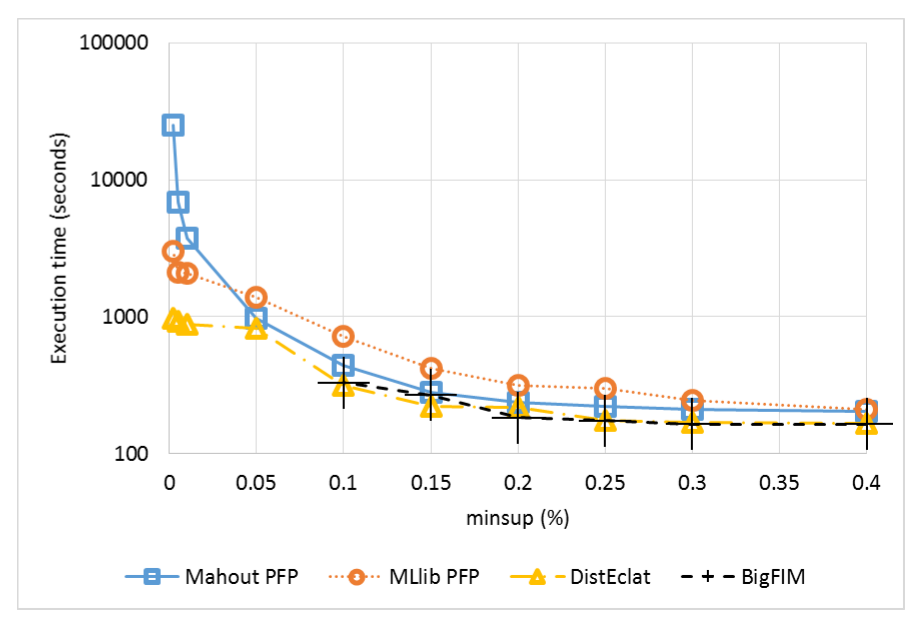
\includegraphics[width=5in]{immagini/minsup_1_log.eps}
\caption{Execution time for different $minsup$ values
(Dataset~\#1), average transaction length~10.}
\label{minsup_1}
\end{figure}


%\begin{figure}[!t]
%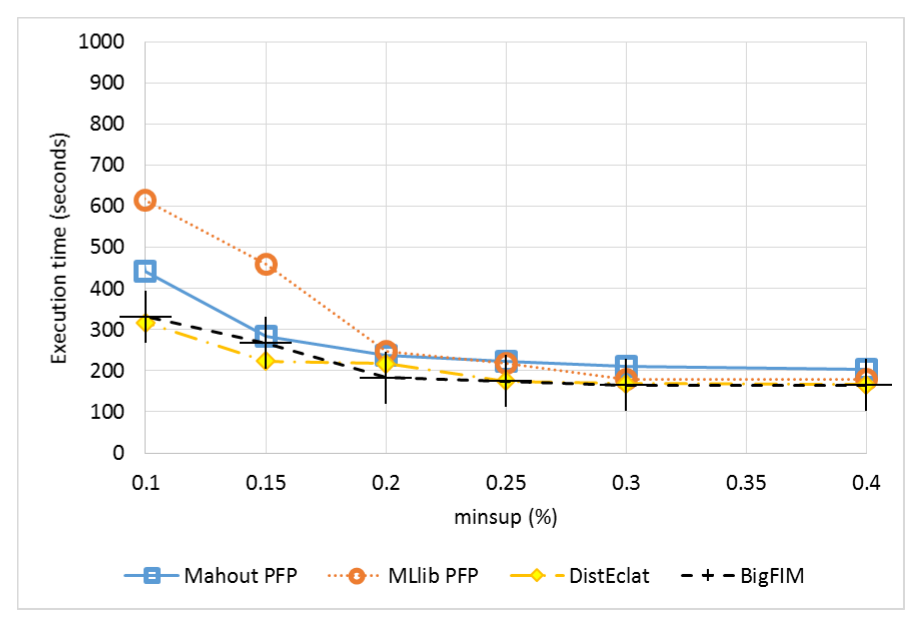
\includegraphics[width=5in]{immagini/minsup_2.eps}
%\caption{Detail of the chart in Figure~\ref{minsup_1} for high $minsup$ values (Dataset~\#1).
%[@FABIO3: da rimuovere, figura precedente ha scala logaritmica.]}
%\label{minsup_2}
%\end{figure}


\begin{figure}[!t]
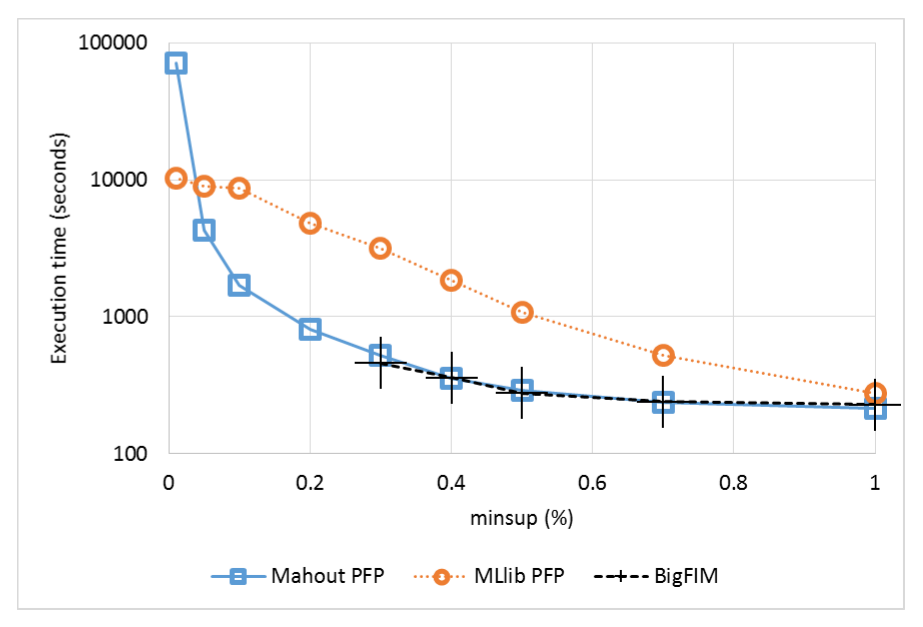
\includegraphics[width=5in]{immagini/minsup_3_log.eps}
\caption{Execution time for different $minsup$ values
(Dataset~\#3), average transaction length~30.}
\label{minsup_3}
\end{figure}



To avoid the bias due to a specific single data distribution,
two different datasets have been considered:
Dataset~\#1 and Dataset~\#3 (Table~\ref{datasets_transactions}).
They share the same average maximal pattern length (5),
the number of different items (100 thousands),
the correlation grade among patterns (0.25), and
the number of transactions (10 millions).
The difference is in the average transaction length:
10 items for Dataset~\#1 and 30 items for Dataset~\#3.
Being the other characteristics constant,
longer transactions lead to a higher dataset density,
which results into a larger number of frequent itemsets.
%Furthermore, we can test the performance degradation
%when dealing with high-dimensional datasets.


Figure~\ref{minsup_1} reports the execution time of the algorithms when varying 
the $minsup$ threshold from 0.002\% to 0.4\% and
considering Dataset~\#1. DistEclat is the fastest algorithm for all the
considered $minsup$ values. However, the improvement with respect to the
other algorithms depends on the value of $minsup$.
%When $minsup$ is greater than or equal to 0.2\%, all the implementations show
%similar performance, with BigFIM and DistEclat being slightly faster than
%Mahout PFP and MLlib PFP.
When $minsup$ is greater than or equal to 0.2\%, all the implementations show
similar performances.
The performance gap largely increases with $minsup$ values lower than 0.05\%.
%Mahout PFP becomes orders of magnitude slower than both
%DistEclat and MLlib PFP. 
BigFIM is as fast as DistEclat when $minsup$ is higher than 0.1\%, but below
this threshold BigFIM runs out of memory during the extraction of 2-itemsets.
%MLlib PFP is generally slower than Mahout PFP,
%becoming faster only for $minsup$ values below 0.05\%.
%Based on this first set of experiments, DistEclat seems to be the
%most appropriate choice, with excellent results when very low values of $minsup$ are considered,
%followed by MLlib PFP, which can reach very low $minsup$ values with
%good performance, at the expense of slightly slower performance for higher $minsup$ values.

% %In this set of experiments, different values of minimum support threshold are
% used to extract the frequent itemsets. The input datasets used are two, with two
% different transaction length: dataset \#1 with 10 items and 10 million
% transactions and dataset \#7, with 30 items and 10 million transactions
% (~\ref{datasets_transactions}).
% %With dataset \#1 and a support above 0,1 \%, all the implementations show
% similar perfomances, as shown in Figure~\ref{minsup_2}, which is an enlargement
% of the the graph in Figure~\ref{minsup_1}. Precisely, BigFIM and DistEclat prove
% to be the fastest implementations. Below this treshold, BigFIM runs out of
% memory, while Mahout PFP completes all the tasks with an execution time much
% higher than the MLlib implementation (almost 6 times).
% % %DistEclat, finally, has the best performance, completing the task with the
% % minimum wallclock time, closely followed by MLlib PFP.
% % %The experiment demostrates that DistEclat and MLlib PFP are the most reliable
% % algorithms when the minsup values start to be very low.

In the second set of experiments, we analyzed the execution time of
the algorithms for different minimum support values on Dataset~\#3,
which is characterized by a higher average transaction length
(3 times longer than Dataset~\#1),
and a larger data size on disk (4 times bigger),
with the same number of transactions (10 millions).
Since the mining task is more computationally intensive,
$minsup$ values lower than 0.01\% were
not considered in this set of experiments,
as this has proven to be a limit for most algorithms
due to memory exhaustion or too long experimental duration (days).
Results are reported in Figure~\ref{minsup_3}.
%DistEclat runs immediately out of memory
%because of the size of the input dataset,
%which is transposed in a vertical format during the first phase:
%the longer transactions prevent it from completing such step.
MLlib PFP is much slower than Mahout PFP for most $minsup$ values (0.7\% and below),
and BigFIM, as in the previous experiment,
achieves top-level performance, but cannot scale to low $minsup$ values
(the lowest is 0.3\%),
due to memory constraints during the $k$-itemset generation phase. Finally, DistEclat was not able to run because the size of the initial tidlists was already too big.\\
Overall, as expected,
DistEclat is the fastest approach when it does not run out of memory.
Mahout PFP is the most reliable implementation across almost all $minsup$ values,
even if it is not always the fastest,
sometimes with large gaps behind the top performers.
MLlib is a reasonable tradeoff choice,
as it is constantly able to complete all the tasks in a reasonable time.
%the 2nd fastest approach
%and it is able to reach the 1st or 2nd lowest $minsup$ values.
Finally, BigFIM does not present advantages over the other approaches,
being unable to reach low $minsup$ values and to provide fast executions. \\
%\textbf{Discussion:} As expected, the first phase of BigFIM is fundamental for its performance. 
%It represents the failure point when the number of candidate itemsets is too large to be stored in the main memory of the mappers. 
%At the same time, thanks to the better load balancing, given by the split of the mining in two phases balanced phases, BigFIM is able to achieve overall competitive performances (when it does not run out of memory in the first phase). Further details about load balancing behaviour can be found in Subsection \ref{load_exp}. While the failures related to mining tasks characterized by deep search space exploration was expected, 
%because of the weakness of breadth-first approach with respect to data density, for the same reasons, the good performances in terms of execution time were less expected. Probably, the competitive performances were caused by the better load balancing in the search space exploration partitioning.\\DistEclat runs easily out of memory because of the size of the input dataset,
%which is transposed in a vertical format during the first phase. 
%The longer tidlists prevent it from completing such step. Even for this algorithm, the first phase is critical. The assumption of storing almost all the input dataset in all the nodes, at the aim of saving reading phases and communication costs, revealed to be not suitable for a problem characterized by a deep search space exploration.\\
%Mahout PFP and MLlib PFP are the only algorithms
%to complete the mining tasks for all $minsup$ values.
%Precisely,
%Mahout PFP is the most suitable technique
%when dealing with minsup values over 0.05\%,
%with a perfomance 6 to 8 times faster than the MLlib sibling.
%However, with lower $minsup$ values,
%Spark MLlib becomes the fastest approach with an order of magnitude gap.
%We identified the cause of the different performance
%between the two PFP implementations
%in the different pruning strategies.
%The algorithms which extract closed itemsets, such as Mahout PFP,
%can apply more effective pruning techniques
%that are not applicable when all frequent itemsets must be extracted,
%which is the case for MLlib PFP.
%When the problem becomes deeper and more challenging, beyond the engineering differences between the two implementations, the better load balancing of the MLlib PFP makes it faster.

%their different mining phases: even if both of them extracts the same set of itemset in this specific use cases, the extraction process is different because MLlib PFP extracts all the frequent itemsets. Mahout PFP, instead, extracts only the closed ones\footnote{The differences are not reported in the paper.}.
%the Spark implementation extracts all the frequent itemsets and then selects the closed ones,
%while the Hadoop implementation directly extracts only the closed frequent itemsets.





% %Indeed, we can say that DistEclat and MLLib are the best approaches for
% different $minsup$ values analyses but are strongly affected, respectively, by
% dataset size and transaction length. When one of these features increases,
% Mahout PFP is the only algorithm able to complete the tasks.

%\begin{table*}[h!]
%\begin{center}
%\caption{Synthetic datasets used for different transaction length experiments}
%\label{datasets_attributes}
%\begin{tabular}{|c|c|c|c|c|}
%\hline
%{\bf ID }& {\bf IBM Generator} &  {\bf \# different } & {\bf  \# items  } & {\bf size} \\
%{\bf  }& {\bf  parameters } &  {\bf items  } & {\bf per } & {\bf (GB) } \\
%{\bf  } & {\bf } & {\bf } & {\bf  transaction } & {\bf } \\ \hline
% \hline
%6  & T20P5I100kC0.25D10000k  & 18011 & 29.99 & 1187 \\ \hline
%7  & T30P5I100kC0.25D10000k  & 18011 & 29.99 & 1776 \\ \hline
%8 & T40P5I100kC0.25D10000k  & 18010 & 39.98 & 2364 \\ \hline
%9 & T50P5I100kC0.25D10000k  & 18014 & 49.98 & 2953 \\ \hline
%10 & T60P5I100kC0.25D10000k  & 18010 & 59.98 & 3541 \\ \hline
%11 & T70P5I100kC0.25D10000k  & 18016 & 69.98 & 4130 \\ \hline
%12 & T80P5I100kC0.25D10000k  & 18012 & 79.98 & 4719 \\ \hline
%13 & T90P5I100kC0.25D10000k  & 18014 & 89.97 & 5307 \\ \hline
%14 & T100P5I100kC0.25D10000k & 18015 & 99.97 & 5896 \\ \hline
%\end{tabular}
%\end{center}
%\end{table*}



%\begin{table*}[h!]
%\begin{center}
%\caption{Synthetic datasets used for different pattern lengths}
%\label{datasets_patterns1}
%\begin{tabular}{|c|c|c|c|c|c|}
%\hline


%{\bf ID }& {\bf IBM Generator parameters } & {\bf Number of } & {\bf Average number of } & {\bf size} \\
%{\bf  } & {\bf } & {\bf different items } & {\bf items per transaction } & {\bf } \\ \hline
% \hline
%15 & T20P2I100kC0.25D10000k  & 8212 & 19,99 & 1.188 \\ \hline
%16 & T20P4I100kC0.25D10000k & 14976 & 19,99 & 1.187 \\ \hline
%17 & T20P6I100kC0.25D10000k  & 20727 & 19,99 &1.187 \\ \hline
%18 & T20P8I100kC0.25D10000k & 25864 & 20,03 &1.188 \\ \hline
%19 & T20P10I100kC0.25D10000k & 30215 & 20,09 &1.192 \\ \hline
%20 & T20P12I100kC0.25D10000k &  34233 & 20,26 &1.202 \\ \hline
%21 & T20P14I100kC0.25D10000k &  37672 & 20,56 & 1.221 \\ \hline
%22 & T20P16I100kC0.25D10000k &  40955 & 21,04 & 1.249 \\ \hline
%
%\end{tabular}
%\end{center}
%\end{table*}






%\begin{table*}[]
%\begin{center}
%\caption{Synthetic datasets used for different pattern lengths}
%\label{datasets_patterns2}
%\begin{tabular}{|c|c|c|c|c|c|}
%\hline
%{\bf ID }& {\bf IBM Generator parameters } & {\bf Number of transactions } & {\bf Number of } & {\bf Average number of } & {\bf size} \\
%{\bf  }& {\bf } & {\bf } & {\bf different items } & {\bf items per transaction } & {\bf } \\ \hline
% \hline
%22 & T40P2I100kC0.25D10000k & 10.000.000 & 8215 & 39,99 & 2,4 GB \\ \hline
%23 & T40P4I100kC0.25D10000k & 10.000.000 & 14,979 & 39,99 & 2,4 GB \\ \hline
%24 & T40P6I100kC0.25D10000k & 10.000.000 & 20733 & 39,98 & 2,4 GB \\ \hline
%25 & T40P8I100kC0.25D10000k & 10.000.000 & 25864 & 39,98 & 2,4 GB \\ \hline
%26 & T40P10I100kC0.25D10000k & 10.000.000 & 30220 & 39,99 & 2,4 GB \\ \hline
%27 & T40P12I100kC0.25D10000k & 10.000.000 & 34262 & 39,98 & 2,4 GB \\ \hline
%28 & T40P14I100kC0.25D10000k & 10.000.000 & 37673 & 39,98 & 2,4 GB \\ \hline
%29 & T40P16I100kC0.25D10000k & 10.000.000 & 40971 & 39,98 & 2,4 GB \\ \hline
%\end{tabular}
%\end{center}
%\end{table*}


%%
%%\begin{table*}[h!]
%%\begin{center}
%%\caption{Experimental result summary for $minsup$ impact, Section~\ref{minsup_exp}}
%%\label{minsup_resume}
%%\begin{tabular}{|c|c|c|c|c|}
%%\hline
%%\textbf{}          & \multicolumn{2}{l|}{\textbf{Transaction length: 10}} & \multicolumn{2}{l|}{\textbf{Transaction length: 30}} \\ \hline
%%\textbf{algorithm} & \textbf{lowest $minsup$}        & \textbf{speed}        & \textbf{lowest $minsup$}        & \textbf{speed}        \\ \hline
%%Mahout PFP         & 0.002 \%                       & 3rd                  & 0.01 \%                         & 2nd                 \\ \hline
%%MLlib PFP          & 0.002 \%                       & 2nd                  & 0.01 \%                         & 1st                  \\ \hline
%%BigFIM             & 0.1 \%                         & 4th        	   & 0.3 \%                         & 3rd                  \\ \hline
%%DistEclat          & 0.002 \%                       & 1st                  & -                              & -                    \\ \hline
%%\end{tabular}
%%\end{center}
%%\end{table*}
%%




\subsection{Impact of the average transaction length}
\label{attributes_exp}

\begin{figure}[!t]
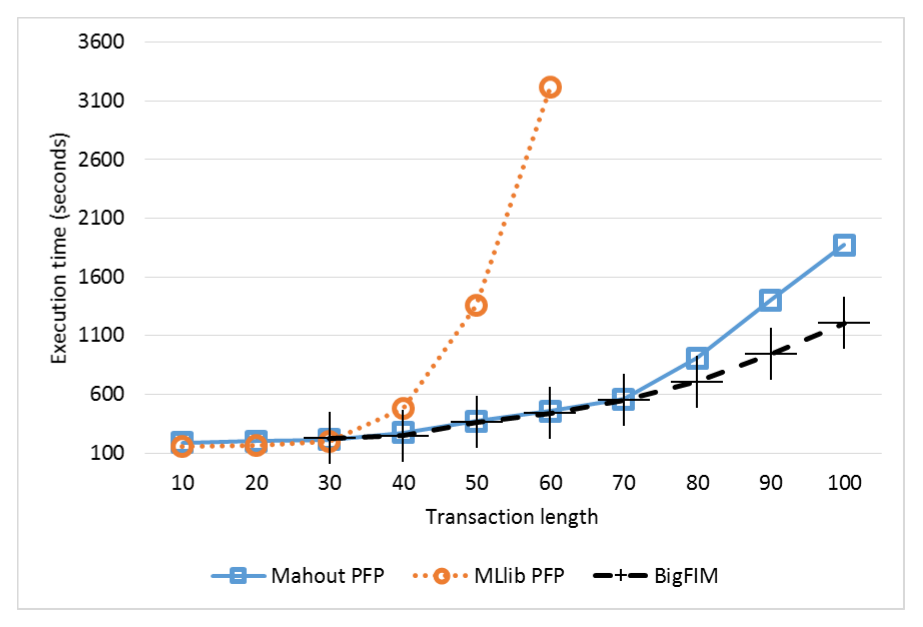
\includegraphics[width=5in]{immagini/attributes.eps}
\caption{Execution time with different average transaction lengths % with a minsup value of 1\%
(Datasets \#1--10, $minsup$ 1\%).}
\label{attributes}
\end{figure}

\begin{figure}[!t]
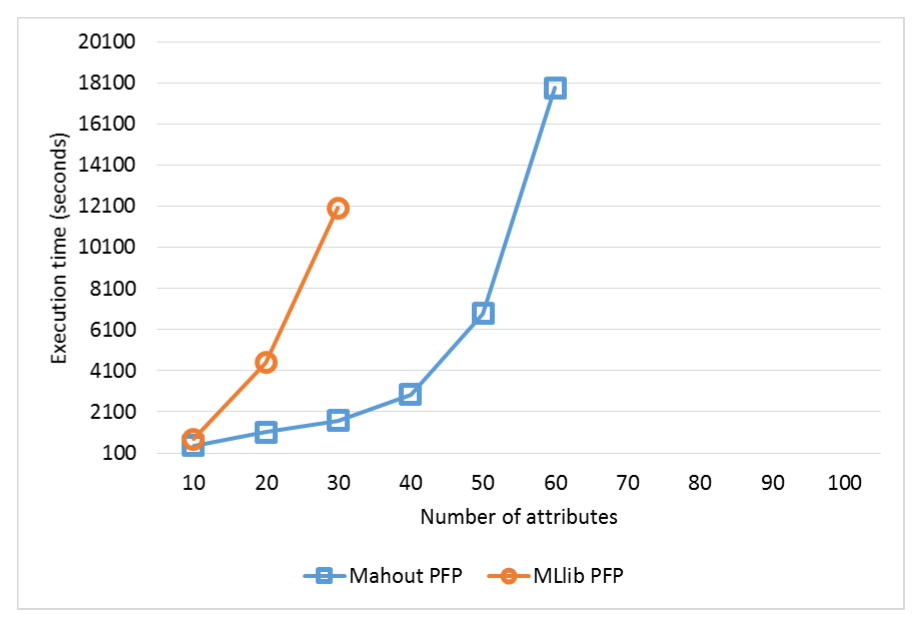
\includegraphics[width=5in]{immagini/attributes_deeper.eps}
\caption{Execution time with different average transaction lengths %with a minsup value of 0.1\%
(Datasets \#1--10, $minsup$ 0.1\%).}
\label{attributes_deeper}
\end{figure}

We analyzed the effect of different average transaction lengths,
from 10 to 100 items per transaction.
We fixed the number of transactions to 10 millions.
To this aim, Datasets \#1--10 were used (see Table~\ref{datasets_transactions}).
Longer transactions often lead to more dense datasets and a larger number of long frequent itemsets.
This generally corresponds to more computationally intensive tasks.
The execution times obtained are reported in Figure~\ref{attributes} and Figure~\ref{attributes_deeper}, with a respective {\it minsup} value of 1\% and 0.1\%.
In the experiment of Figure~\ref{attributes}, BigFIM and DistEclat execution times for transaction length of 10 and 20 are not reported because, for these configurations, no 3-itemsets are extracted and hence the two algorithms crashed\footnote{Due to the absence of a specific test, BigFIM and DistEclat crash
if no itemsets longer than the value of the prefix length parameter are mined.}.
For higher transaction lengths, DistEclat is not included since it runs out of memory
for values beyond 20 items per transaction.
The other algorithms have similar execution times for short transactions,
up to 30 items.
For longer transactions, a clear trend is shown:
(i) MLlib PFP is much slower than the others
and it is not able to scale for longer transactions,
as its execution times abruptly increase until it runs out of memory;
(ii) Mahout PFP and BigFIM have a similar trend until 70 items per transactions,
when Mahout PFP becomes slower than BigFIM.\\
The experiments of Figure~\ref{attributes_deeper}, shows a very similar trend, with exception that also BigFIM is not able to run.\\
Overall, despite the Apriori-based initial phase,
BigFIM proved to be the best scaling approach for very long transactions and a relatively high minsup. When the minsup is decreased only Mahout PFP 
is able to cope with the complexity of the task.\\
%\textbf{Discussion:} As expected (see Figure~\ref{attributes_deeper}), for more dense data distributions the number of candidate itemsets increases and BigFIM runs out of memory due to its initial Apriori phase. 
%A similar motivation holds for DistEclat failures, due to its requirement to store all the (longer) tidlists in all the nodes.
%The FP-growth based approaches are affected by the increasing length of the transactions. However, their depth-first structure revealed to be the best exploration strategy in such an environment (i.e. high number of attributes). 
%DistEclat leverages a depth-first exploration strategy as well, however it assumes that all the tidlists should be stored in all the commodity cluster nodes, which is challenging if considering the further memory requirements due to the search space exploration. 
%The difference gap between the two PFP implementations might be related to the different pruning strategies.


%Despite the Apriori-based initial phase, BigFIM shows to be the mo
%PFP is not optmized to address long transactions due to its FP-tree structure,
%whereas BigFIM is able to address denser data distributions and a large
%number of attributes.


%\begin{table*}[h!]
%\begin{center}
%\caption{Experimental result summary for transaction length impact, Section~\ref{attributes_exp}}
%\label{transaction_length_resume}
%\begin{tabular}{|c|c|c|}
%\hline
%
%\textbf{algorithm} & \textbf{reached transaction length}        & \textbf{speed}        \\ \hline
%BigFIM             & 100                        & 1st        	                  \\ \hline
%Mahout PFP         & 100                       & 2nd                          \\ \hline
%MLlib PFP          & 60                       & 3rd                                 \\ \hline
%DistEclat          & -                       & -                            \\ \hline
%\end{tabular}
%\end{center}
%\end{table*}
%


% % COMMENTO A FIGURA 5 RIMOSSA
% In order to assess this type of experiments with the ones of the Section
% \ref{minsup_exp}, we have performed a set of experiments dealing with datasets
% of both a varying transaction length (focusing on datasets with an average
% number of items from 10 to 30) and different minsup values (0.01\% and 0.05\%).
% % %We also performed a set of experiments with the same datasets lowering the
% % minimum support threshold (we considered $minsup$=0.01\% and $minsup$=0.05\%) .
% The results are reported in Figure \ref{attributes_2}.  The execution time of
% BigFIM is not reported because, as already evidenced in Section
% \ref{minsup_exp},  it is unable to complete the mining task when
% low values of minsup are considered. On the other hand, different performances
% of Mahout PFP and MLlib PFP are noticeable. When the $minsup$ is 0.05\% Mahout
% PFP is
% still faster than MLlib PFP. Indeed, when the $minsup$ value is 0.01\% MLlib
% becomes faster
% than Mahout PFP. Hence, this results confirm that MLlib is the best approach
% when dealing with very low $minsup$ values.




% %The difference between the performance of Mahout PFP and MLlib PFP, as before,
% may be caused by the difference mining processes. Since Mahout PFP
% %mines only the frequent closed itemsets, it can exploit more effective pruning
% techniques and reduce the depth of the recursive mining phase. Differently,
% %MLlib PFP, which mines all the frequent itemsets, has a deeper recursive mining
% phase, in particular when long transactions are considered.
% %The difference between the performance of Mahout PFP and MLlib PFP, as before,
% may be caused by the difference mining processes which lead to different type
% %of outputs, even if, in this specific case, the number of frequent itemsets
% matches the number of closed ones.



% \begin{figure}[!t]
% 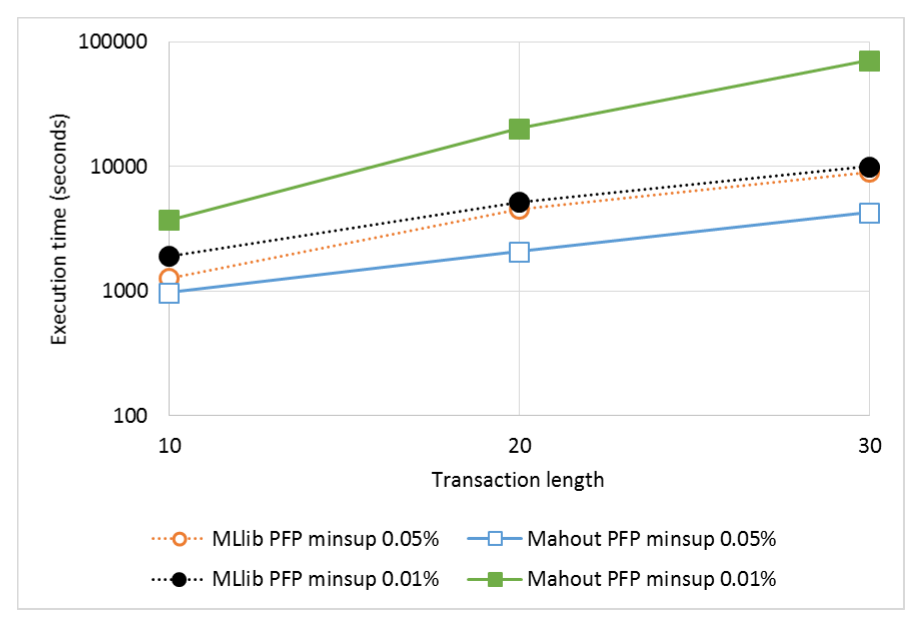
\includegraphics[width=5in]{immagini/attributes_2.eps}
% \caption{Execution time with different average transaction lengths,
% and $minsup$ values 0.01\% and 0.05\%.}
% \label{attributes_2}
% \end{figure}



% %ELIMINARE DA QUI
% %The second set of experiments studies the performance of the approaches dealing
% with datasets obtained setting different expected frequent patterns length. We
% utilised a configuration with 20 attributes and another with 40 (respectively
% detailed in tables ~\ref{datasets_patterns1} and ~\ref{datasets_patterns2}) with
% different expected patterns length. Therefore, the datasets of these evaluation
% differ for their density. A higher expected pattern length is typical of dense
% dataset distributions, while sparse datasets are characterised by many short
% itemsets.
% %The minsup value is set to 0,25\% for the first set of experiments and to
% 0,40\% for the second one. We changed the minsup values in order to have
% significative output and a good number of approaches that not run out of memory.
% %
% %In the first case, DistEclat was able to run even if it showed memory issues
% for the longest expected patterns, as illustrated in the graph in
% Figure~\ref{pattern_small}. Even in this experiment, BigFIM performances
% revealed to be the most stable of the set of algorithms for all the pattern
% length configurations, even if Mahout PFP is not far. MLlib implementation is
% able to execute all the tasks, but it shows a serious gap when the expected
% patterns are short. This is very interesting, because one can expect a behaviour
% more similar to the one of the previous experiment, where the execution time
% strongly increases together with the average transaction length of the input
% dataset. Clearly, the perforamance related to the average length of transactions
% and the average length of the expected patterns are not correlated.
% %We counted the frequent itemsets produced to understand if the performance
% degradation was reasoned by an explosion of the number of itemsets. As repored
% in Table~\ref{extracted_itemsets}, this was not the case.
% %
% %In the second case, with an average transaction length of 40 items and a minsup
% of 0,4\%, the behaviour of the algorithms is very similar, except for DistEclat
% that is not able to mine the input. BigFIM shows the best performance followed
% by Mahout PFP, which has apeak corresponding to an expected pattern length of
% 14. The behaviour is similar to the previous experiment, in which it was less
% explicit. In these cases, the number of extracted itemset is much higher than
% the previous case, as shown in Table~\ref{extracted_itemsets}. Above all, the
% high execution time is caused by a not proper load balancing. In fact, almost
% all the tasks of the mining MapReduce job of the process finish the computation
% below a minute of wall clock time, one of them reaches 3 minutes while the last
% 2 last respectively take over 8 minutes and over 32 minutes. This validates the
% assumption about Mahout PFP load balancing in subSection ~\ref{FP-Growth}.
%




%\begin{table*}[h!]
%\begin{center}
%\caption{Synthetic datasets used for different pattern lengths}
%\label{datasets}
%\begin{tabular}{|c|c|c|c|c|c|}
%\hline
%
%ID & IBM Generator  & Number of  & Number of  & Average number & size\\
% & parameters & transactions & different & of items per & \\
% & &  &  items & transaction &\\ \hline
%14 & T20P2I100kC0.25D10000k & 10.000.000 & 8212 & 19,99 & 1,2 GB \\ \hline
%15 & T20P4I100kC0.25D10000k & 10.000.000 & 14976 & 19,99 & 1,2 GB \\ \hline
%16 & T20P6I100kC0.25D10000k & 10.000.000 & 20727 & 19,99 & 1,2 GB \\ \hline
%17 & T20P8I100kC0.25D10000k & 10.000.000 & 25864 & 20,03 & 1,2 GB \\ \hline
%18 & T20P10I100kC0.25D10000k & 10.000.000 & 30215 & 20,09 & 1,2 GB \\ \hline
%19 & T20P12I100kC0.25D10000k & 10.000.000 & 34233 & 20,26 & 1,2 GB \\ \hline
%20 & T20P14I100kC0.25D10000k & 10.000.000 & 37672 & 20,56 & 1,2 GB \\ \hline
%21 & T20P16I100kC0.25D10000k & 10.000.000 & 40955 & 21,04 & 1,2 GB \\ \hline
%
%\end{tabular}
%\end{center}
%\end{table*}
%
%\begin{table*}[h!]
%\begin{center}
%\caption{Synthetic datasets used for different pattern lengths}
%\label{datasets}
%\begin{tabular}{|c|c|c|c|c|c|}
%\hline
%
%ID & IBM Generator  & Number of  & Number of  & Average number & size\\
% & parameters & transactions & different & of items per & \\
% & &  &  items & transaction &\\ \hline
%22 & T40P2I100kC0.25D10000k & 10.000.000 & 8215 & 39,99 & 2,4 GB \\ \hline
%23 & T40P4I100kC0.25D10000k & 10.000.000 & 14,979 & 39,99 & 2,4 GB \\ \hline
%24 & T40P6I100kC0.25D10000k & 10.000.000 & 20733 & 39,98 & 2,4 GB \\ \hline
%25 & T40P8I100kC0.25D10000k & 10.000.000 & 25864 & 39,98 & 2,4 GB \\ \hline
%26 & T40P10I100kC0.25D10000k & 10.000.000 & 30220 & 39,99 & 2,4 GB \\ \hline
%27 & T40P12I100kC0.25D10000k & 10.000.000 & 34262 & 39,98 & 2,4 GB \\ \hline
%28 & T40P14I100kC0.25D10000k & 10.000.000 & 37673 & 39,98 & 2,4 GB \\ \hline
%29 & T40P16I100kC0.25D10000k & 10.000.000 & 40971 & 39,98 & 2,4 GB \\ \hline
%\end{tabular}
%\end{center}
%\end{table*}




\subsection{Impact of the number of transactions}
\label{transaction_exp}

\begin{figure}[!t]
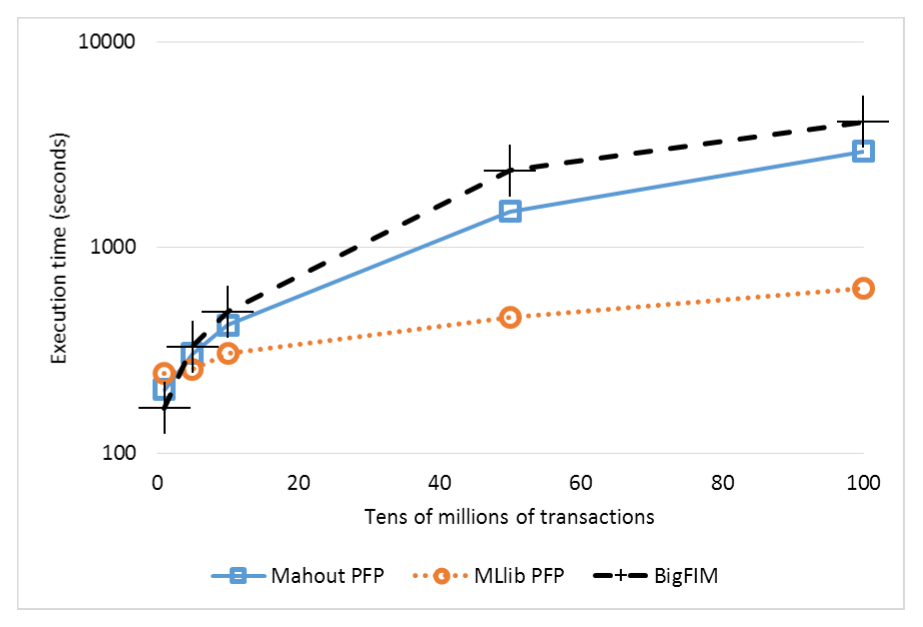
\includegraphics[width=5in]{immagini/transactions_log.eps}
\caption{Execution time with different numbers of transactions
 (Datasets \#1, \#11--14,
 $minsup$~0.4\%).}
\label{transactions}
\end{figure}

We evaluated the effect of varying the number of transactions,
i.e., the dataset size, without changing intrinsic data characteristics (e.g., 
transaction length or data distribution).
The experiments have been performed on Datasets \#1, \#11--14 have been used
(see Table~\ref{datasets_transactions}),
which have a number of transactions
ranging from 10 millions to 1 billion.
The $minsup$ is set to 0.4\%,
which is the highest value for which the mining leverages both the two phases of
BigFIM, and it corresponds to the highest value used
in the experiments of Section~\ref{minsup_exp}.
Since in the experiment the relative minsup threshold is fixed, from the mining point of view, the search space exploration is similar and not particularly challenging, as shown in Section~\ref{minsup_exp}. What really affects this experiment is the algorithms reliability dealing with such amount of data.

As shown in Figure~\ref{transactions}, all the considered algorithms scale
almost linearly with respect to the dataset cardinality, with BigFIM being the slowest,
closely followed by Mahout PFP,
and with MLlib PFP being by far the fastest approach,
with execution times reduced by almost an order of magnitude. 
PFP implementations are faster than BigFIM because they read from the disk the input dataset only twice. 
BigFIM pays the iterative disk reading activities during its initial Apriori phase when the number of records
of the input dataset increases.
Finally, DistEclat fails under its assumption that the tidlists of the entire dataset should
be stored in each node, and it is not able to complete the extraction beyond
10 million transactions.
%This experiment, because of the size of the involved input dataset, should be very related to the behavior in terms of communication costs of the algorithms. As we will detail in Subsection~\ref{communication_costs}, Mahout PFP implemention is, by far, the algorithm assuming less data across the network. However, in this experiment, the performance of Mahout PFP are not the best-in-class. For the same reason, even the gap with the performances of BigFIM is not that large (since the communication costs balance differs, instead, by a factor larger than four).
%\begin{table*}[h!]
%\begin{center}
%\caption{Experimental result summary for number of transactions impact, Section~\ref{transaction_exp}}
%\label{transaction_resume}
%\begin{tabular}{|c|c|c|}
%\hline
%
%\textbf{algorithm} & \textbf{reached dataset size}        & \textbf{speed}      \\
%\textbf{algorithm} & \textbf{tens of millions of transactions}        &      \\ \hline
%MLlib PFP          & 100                       & 1st                               \\ \hline
%Mahout PFP         & 100                       & 2nd                          \\ \hline
%BigFIM             & 100                        & 3rd       	                  \\ \hline
%DistEclat          & 1                       &  -                            \\ \hline
%\end{tabular}
%\end{center}
%\end{table*}








\subsection{Scalability in terms of parallelization degree}
\label{nr_machines}



\begin{figure*}[!t]
\begin{center}
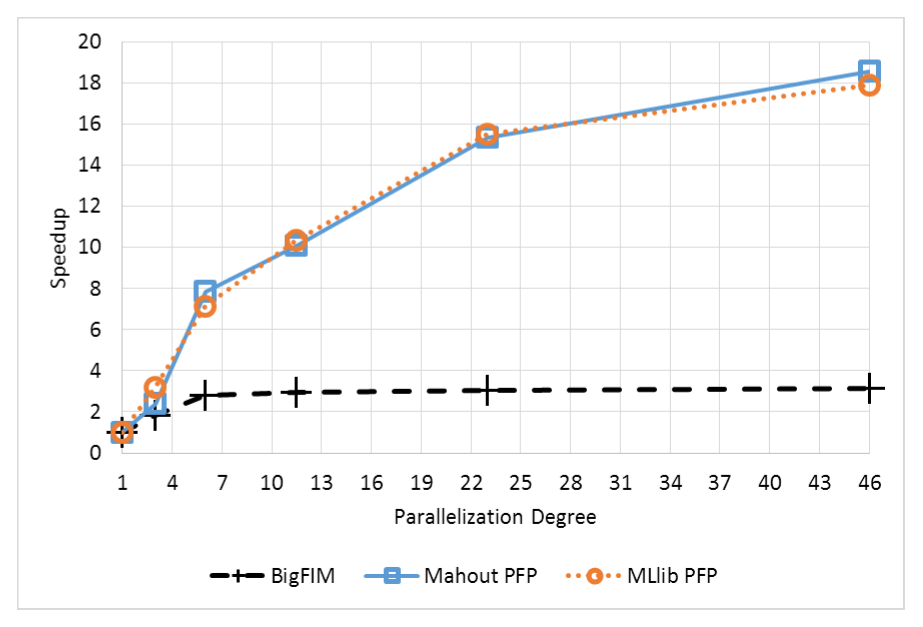
\includegraphics[width=5in]{immagini/machines_big.eps}
\caption{Speedup with different parallelization degrees (Dataset \#14,
 $minsup$~0.4\%)}
\label{nr_machines_speedup}
\end{center}
\end{figure*}


%\begin{figure*}[!t]
%\begin{center}
%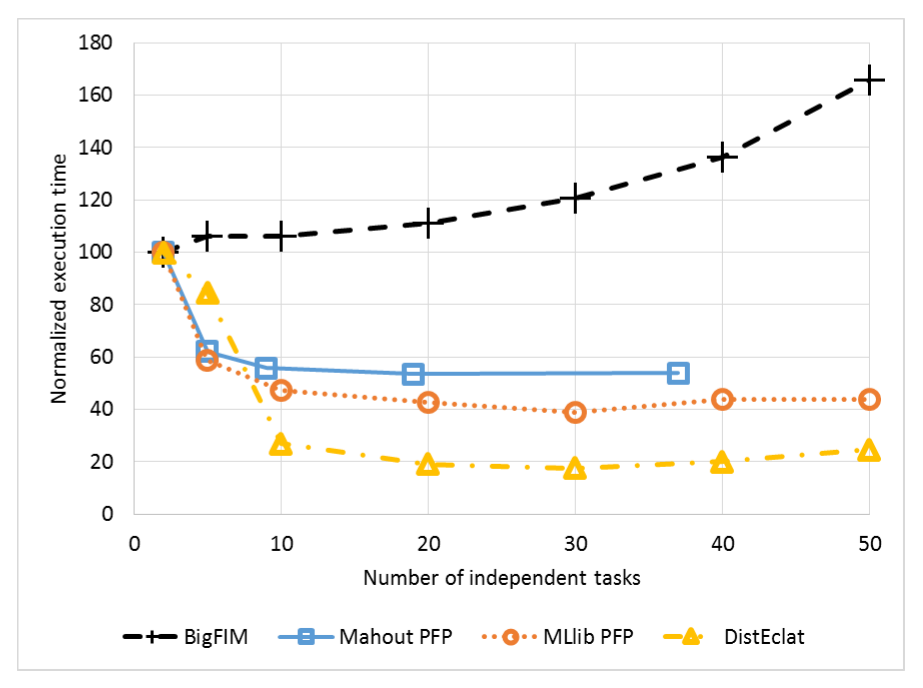
\includegraphics[width=5in]{immagini/machines_2.eps}
%\caption{Normalized execution time with different number of machines  (Dataset \#1,
% $minsup$~0.11\%,
% average transaction length~10) \textbf{Qui BigFIM va proprio male, mi chiedo se sia il caso di eliminare questo esperimento (ma perderemmo disteclat)}}
%\label{nr_machines_2}
%\end{center}
%\end{figure*}

We analyzed the speedup by running the same mining problem with increasing numbers of parallel tasks.
The dataset selection and the $minsup$ parameter choice are difficult 
since we need to identify a mining problem satisfying two conditions:
(i) allowing all the executions to complete with any number of parallel tasks, 
and, at the same time, 
(ii) being very demanding so that the distributed framework is actually exploited. 
We selected $minsup$ 0.4\% and Dataset \#14 (see Table~\ref{datasets_transactions}) 
to be light enough for condition (i) and demanding enough for condition (ii).

Figure~\ref{nr_machines_speedup} shows the speedup results. 
A parallelization degree equal to 1 corresponds to the minimal computational resource setting, i.e., the configuration with only two parallel independent tasks.
Its execution time is the reference with respect to which the speedup is computed. 
Specifically, the speedup of a configuration with a parallelization degree equal to $p$ is computed as 

$$speedup(paral\_degree=p)=\frac{Exec\_Time(paral\_degree=1)}{Exec\_Time(paral\_degree=p)}$$. 

Ideally, the speedup should be equal to the parallelization degree $p$ itself, i.e., 
increasing the number of resources (parallel tasks) of a factor $p$, should lead to a speedup equal to $p$.
%In Figure~\ref{nr_machines_speedup}, the execution time of the basic configuration are divided by the ones related to the higher degree of parallelization to obtain the speedup values.
 % (Figure~\ref{nr_machines_1}). 
%Since the problem was already too challenging for a single task, we have started from 2. In Figure~\ref{nr_machines_1} and Figure~\ref{nr_machines_speedup} are shown the performance of the algorithms leveraging different parallelization degree values.
% In In Figure~\ref{nr_machines_1}, the execution times are normalized with respect with the execution time obtained with the time obtained with the base number of machines (i.e. 2).
% ( $T_{old}/T_{new}$ ).
%for different multiplicative factors of computation improvement (since the basic parallelization degree is 2, the number of independent tasks in the x axis can be obtained by multiplying times 2)     \footnote{Please note that the Mahout-PFP curve in Figure~\ref{nr_machines_1} appears shifted with respect to the others because of the following reason. This specifical implementation does not allow to control the numbers of mappers involved in the computation, therefore we had to change input chunk size. This value allowed us to force a fixed set of possible configurations. }. 

In this experiment, it is clear that the FP-Growth-based implementations provide a better speedup. 
BigFIM, on the contrary, is not able to leverage a number of parallel tasks higher than 6.
% However, only MLlib PFP has a speedup that is close to the ideal one.
Because of the size of the dataset, DistEclat is not able to perform the mining. 
%In the previous experiments, it has demonstrated to be reliable only with mining requiring less than few minutes \footnote{Considering just the experiments in which all the algorithms complete the mining}. Repeating the same kind of scalability experiment for a mining of few minutes is not sensed because the parallelization overheads likely dominate the computation.\\
%
%Since DistEclat is not able to run this experiment, we used a smaller input file (Dataset \#1) and an even lower minsup value (0.11\%) (Figure~\ref{nr_machines_2}). Even in this case, the Breadth-first approaches (DistEclat) showed a very good scalability. BigFIM demonstrated again to have serious problems of scalability. In this experiment, in fact, the problem configuration is such that the best execution times is provided with the smaller number of computing nodes. Actually, the mining phase is quite fast (about 6 minutes), with a concrete possibility, hence, to be dominated by distribution overheads, especially with Apriori iterative nature. However, a slightly deeper minsup value leads to memory issue.\\
%\textbf{Discussion:}
%Based on the results it is clear that many of the considered algorithms are not able to properly exploit the parallelism provided by distributed frameworks. The reason 
%is probably given by the fact that they are not able to split the initial problem in a number of subproblems equal to the number of available parallel 
%tasks, or, when they are able to do so, the overhead given by the instance of the subtasks is greater than the advantages given by the parallel execution 
%of the subtasks/subproblems. 
%MLlib PFP has demonstrated to be the best approach, probably because of a finest granularity in the projection of the FP-trees than the other FP-growth-based approaches (the more are the independent subproblems generated, the better could be distributed to a high number of nodes). 
%Based on the results it is clear that many of the considered algorithms are not able to properly exploit the parallelism provided by Hadoop. The reason 
%is probably given by the fact that they are on able to split the initial problem in a number of subproblems equal to the number of available parallel 
%tasks, or when they are able to do it, the overhead given by the instance of the subtasks is greater than the advantages given by the parallel execution 
%of the subtasks/subproblems. MLlib PFP has demonstrated to be the best approach, probably because of a finest granularity in the projection of the FP-trees than the other FP-growth-based approaches (the more are the independent subproblems generated, the better could be distributed to a high number of nodes). 




%In this Section, as predictable, it is clear that the benefits of the parallelization is strongly mitigate after few tens of tasks. MLlib PFP has demonstrated to be the best approach, probably because a finest granularity in the projection of the FP-trees than the other approaches tree structures (the more are the independent structures to be mined, the better could be distributed to a high number of nodes). 
%The motivations behind this difficulties are related to the Frequent itemset mining problem, which is hardly parallelizzable. The partitions to which the problem is divided into often overlap. This leads to an overall load which is higher than load of an hypothetical centralized execution. For this reason, when the exploration of the search space deepen, the overlapping of the subproblems increases and the performances do not scale as desirable. 
%\textbf{(ANCHE QUI FORSE POTREMMO ENFATIZZARE IL FATTO CHE PURTROPPO IN QUESTO DOMINIO SI SCALA DAVVERO POCO. NON CONTINUARE A GUADAGNARE ALL'INFINITO E' LA NORMA, MA QUI ANCHE PROBLEMI MOLTO GRANDI SI FERMANO DOPO QUALCHE DECINE DI MACCHINE. CI POTREMMO ALLACCIARE ALLE RIFLESSIONI FINALI IN CUI DICIAMO CHE SI VEDE CHE QUESTI SONO PORTING E NESSUNO E' STATO DAVVERO PROGETTATO PER ANDARE DIRETTAMENTE PARALLELO.}


\subsection{Real use cases}
\label{usecases}

In the following, we analyze the performance of the mining algorithms in two
real-life scenarios:
(i) URL tagging of the Delicious dataset and
(ii) network traffic flow analysis.
The characteristics of the two datasets
are reported in Table~\ref{datasets_real}.

\begin{table*}[h!]
\scriptsize
\begin{center}
\caption{Real-life use-cases dataset characteristics}
\label{datasets_real}
\begin{tabular}{|c|c|c|c|c|c|}
\hline
{\bf ID }& {\bf Name} 	&  {\bf Num. of} 	& {\bf  Avg. \# items} 			& {\bf Size} \\
{\bf  }& {\bf  } 		&  {\bf different items} 	& {\bf  per transaction} 	& {\bf (GB) } \\
\hline
\hline
15& Delicious & 57,372,977 & 4 & 44.5 \\ \hline
16 & Netlogs & 160,941,600 & 15 & 0.61  \\ \hline
\end{tabular}
\end{center}
\end{table*}





\subsubsection{URL tagging}
\label{delicious_exp}

We evaluated the selected algorithms on the Delicious dataset~\cite{wetzker2008analyzing}, which is a
collection of web tags.
Each record represents the tag assigned by a user to a URL and it consists of
4 attributes:
date,
user id (anonymized),
tagged URL,
and tag value.
The transactional representation of the Delicious dataset includes
one transaction for each record, where each transaction is a set of four pairs
(attribute, value), i.e., one pair for each attribute.
The dataset stores more than 3 years of web tags.
It is very sparse because of the huge number of different URLs
and tags.
Additional characteristics of the dataset are reported
in Table~\ref{delicious_itemsets}.

This experiment simulates the environment of a service provider that
periodically analyzes the web tag data to extract frequent patterns: they
represent the most frequent correlations among tags, URLs, users, and dates.
Many different use cases can fit this description:
tag prediction, topic classification, trend evolution, etc.
Their evolution over time is also interesting.
To this aim, the frequent itemset extraction has been executed
cumulatively on temporally adjacent subsets of data,
whose length is a quarter of year (i.e., first quarter,
then first and second quarter, then first, second, and third quarter, and so on,
as if the data were being colleted quarterly and analyzed as a whole at the
end of each quarter).
The setting of $minsup$ in a realistic use-case proved to be a critical choice.
Too low values lead to millions of itemsets,
which become useless as they exceed the human capacity to understand the results.
However, too high $minsup$ values would discard longer itemsets,
which are more meaningful
as they better highlight more complex correlations
among the different attributes and values.
Because of the high sparsity of the dataset,
we identified the setting $minsup$=0.01\% as the best tradeoff.

\begin{table}[h]
\scriptsize
\begin{center}
\caption{Delicious dataset: cumulative number of transactions and frequent itemsets
with $minsup$~0.01\%.}
\label{delicious_itemsets}
\begin{tabular}{|c|c|c|c|}
\hline
{\bf Up to year,}	& {\bf Number of} 	& {\bf	Number of} \\
{\bf month, quarter}	& {\bf transactions} 	& {\bf	frequent itemsets} \\
\hline \hline
2003 Dec, Q4 	& 153,375	 	& 7197 \\ \hline
2004 Mar, Q1  	& 489,556		& 6013 \\ \hline
2004 Jun, Q2	& 977,515		& 5268 \\ \hline
2004 Sep, Q3 	& 2,021,261		& 5084 \\ \hline
2004 Dec, Q4 	& 4,349,209		& 4714 \\ \hline
2005 Mar, Q1	& 9,110,195		& 4099 \\ \hline
2005 Jun, Q2	& 15,388,516		& 3766 \\ \hline
2005 Sep, Q3	& 24,974,689		& 3402 \\ \hline
2005 Dec, Q4	& 41,949,956		& 3090 \\ \hline
\end{tabular}
\end{center}
\end{table}

\begin{figure}[!t]
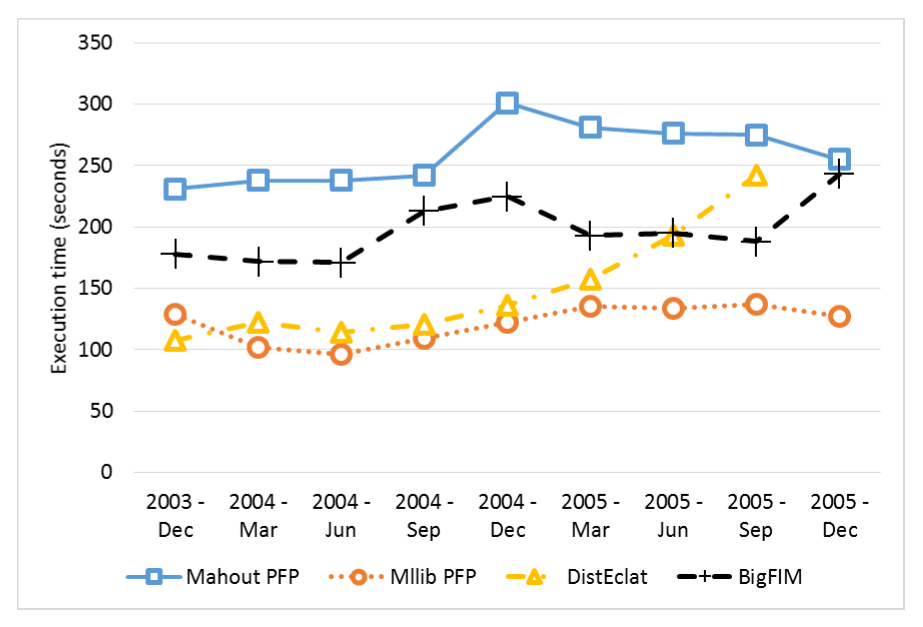
\includegraphics[width=5in]{immagini/delicious.eps}
\caption{Execution time for different periods of time on the Delicious dataset
($minsup$=0.01\%)}
\label{delicious}
\end{figure}


Table~\ref{delicious_itemsets} reports the cumulative number of
transactions for the different periods of time
(i.e., the cardinality of the input dataset) and the
number of frequent itemsets extracted with a fixed $minsup$ of 0.01\%,
while the execution times of the
different algorithms are shown in Figure~\ref{delicious}.


MLlib PFP consistently proves to be the fastest approach, with DistEclat following.
However, while DistEclat is slightly faster than MLlib PFP only with the first, smallest dataset
(up to Dec 2003, with 150 thousands transactions), when the dataset size increases,
DistEclat execution time does not scale. DistEclat eventually fails for the final
40-million-transaction dataset of Dec 2005, due to memory exhaustion.
BigFIM and Mahout PFP consistently provide 2 to 3 times higher execution times.
Apart from DistEclat, all algorithms complete the task with similar performance
despite increasing the dataset cardinality from 150 thousand transactions to 41 millions,
thanks to the constant relative $minsup$ threshold
which reduces the number of frequent itemsets
for decreasing density of the dataset.
Hence, MLlib PFP is the best choice for this dataset characterized by short transactions
(the transaction length is 4).


% %Therefore, we extracted the frequent itemset related to an incremental period
% of time covering 4 years of tags.
% %For this scope, we were forced to change the minsup values in some experiments.
% The choice of the minsup value strongly impacts the results. On one hand we did
% not want to want to extract a billion of itemsets, because they would not be
% realistically processable. On the other hand, we did not want just a list of
% items (header table) which can be obtained with the most trivial Word Count
% MapReduce implementation. Furthermore, we wanted to obtain at least some
% 3-itemsets in order to exploit the BigFIM two phases, without reducing it to a
% pure DistEclat.
% %
% %The choice was made harder by the dataset sparsity. Adding a new period of time
% to the computation corresponds to new transactions in the input datasets.
% However, adding new transactions means adding new items of such a sparse
% dataset. In few words, the sparsity of the input dataset grows up faster than
% the number of transactions. Consequently, the same minimum support thresholds
% for each scrape of dataset would not always carry to the desired ouput. It would
% lead to a very intensive task and a very high number of frequent itemsets when
% the transactions are few; it would not result low or deep enough to extract a
% significative number of itemset when the number of transactions is high, because
% of the sparsity of the dataset. For this reason, we deepened the minsup value
% for the computation related to the transaction related to the last year of tags,
% as shown in Table~\ref{delicious_itemsets}.
% %The execution time of the different algorithms are shown in the graph in
% Figure~\ref{delicious}. DistEclat revealed to be the most performant approach
% before running out of memory. This is something unexpected because the
% depth-first search strategy hardly fits sparse dataset distributions. BigFIM
% outperforms Mahout PFP while MLlib implementation revealed to be the most
% reliable solution, with an almost flat curve.



%\begin{table}[h]
%\begin{center}
%\caption{Number of tags for year and minsup used for Delicious}
%\label{delicious_itemsets}
%\begin{tabular}{|c|c|c|c|}
%\hline
%{\bf Year }	& {\bf Tags} & {\bf minsup (\%) } & {\bf	frequent itemsets } \\ \hline \hline
%2003	& 153375	 & 0.01 &	7197 \\ \hline
%2004 &	4195834	& 0.01	& 4714 \\ \hline
%2005	& 37600747	& 0.01	& 3090 \\ \hline
%2006	& 130799274	& 0.005 &	5321 \\ \hline
%\end{tabular}
%\end{center}
%\end{table}





\subsubsection{Network traffic flows}
\label{net_exp}


\begin{figure}[!t]
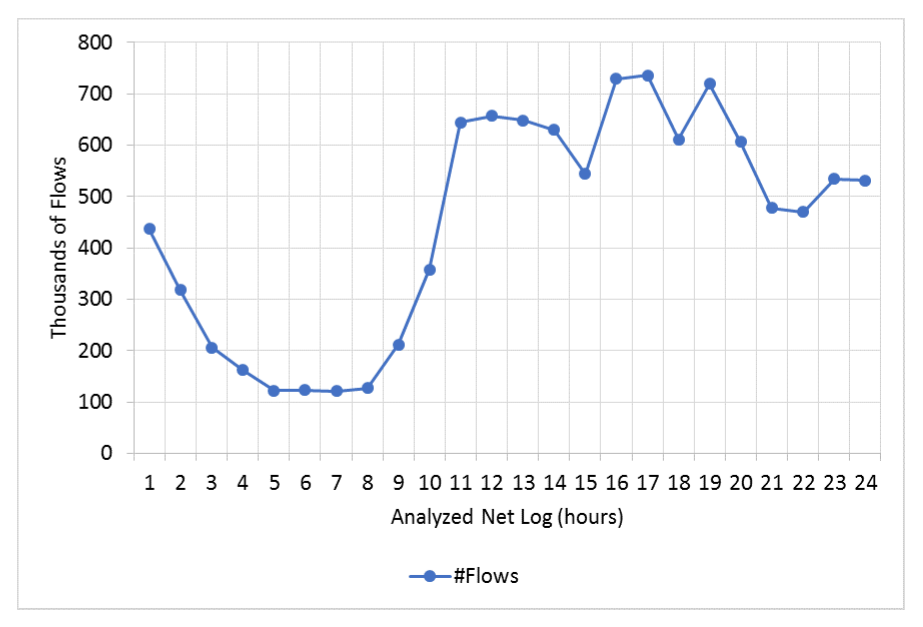
\includegraphics[width=5in]{immagini/number_flows.eps}
\caption{Number of flows for each hour of the day.}
\label{number_flows}
\end{figure}

\begin{figure}[!t]
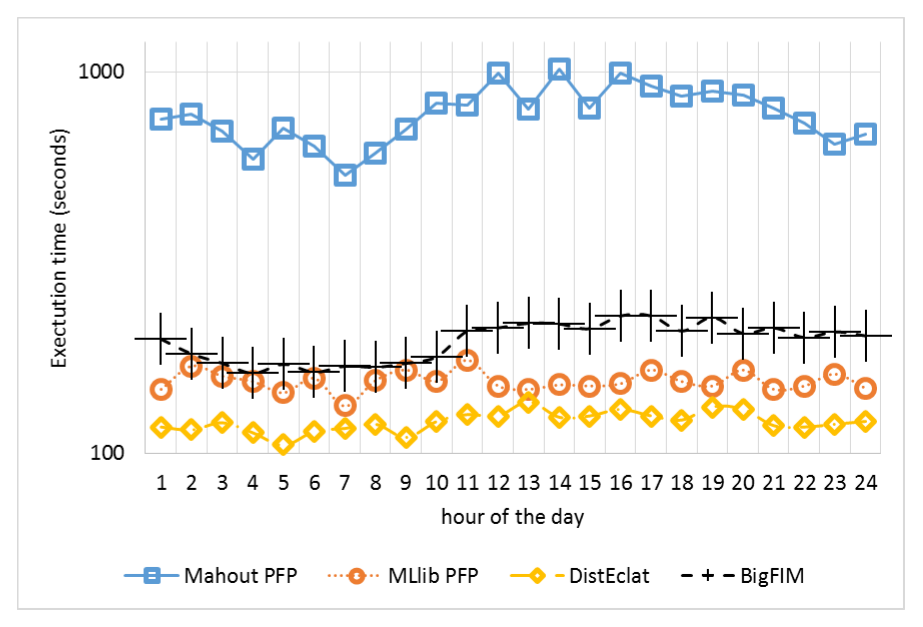
\includegraphics[width=5in]{immagini/net_logs_log.eps}
\caption{Execution time of different hours of the day.
(dataset 31, $minsup$=1\%)}
\label{net}
\end{figure}


\begin{table}[h!]
\scriptsize
\begin{center}
\caption{Network traffic flows: number of transactions and frequent itemsets
with $minsup$~0.1\%.}
\label{netlog_itemsets}
\begin{tabular}{|c|c|c|}
\hline
{\bf Hour of}	& {\bf Number of} 	& {\bf	Number of} \\
{\bf the day}	& {\bf transactions} 	& {\bf	frequent itemsets} \\
\hline \hline
0.00  & 437,417 & 166,217 \\ \hline
1.00  & 318,289 & 173,960 \\ \hline
2.00  & 205,930 & 163,266 \\ \hline
3.00  & 162,593 & 166,344 \\ \hline
4.00  & 122,102 & 157,069 \\ \hline
5.00  & 123,683 & 164,493 \\ \hline
6.00  & 121,346 & 170,129 \\ \hline
7.00  & 127,056 & 159,921 \\ \hline
8.00  & 211,641 & 169,751 \\ \hline
9.00  & 357,838 & 187,912 \\ \hline
10.00 & 644,408 & 191,867 \\ \hline
11.00 & 656,965 & 183,021 \\ \hline
12.00 & 648,206 & 184,279 \\ \hline
13.00 & 630,434 & 180,384 \\ \hline
14.00 & 544,572 & 175,252 \\ \hline
15.00 & 729,518 & 192,992 \\ \hline
16.00 & 735,850 & 189,160 \\ \hline
17.00 & 611,582 & 177,808 \\ \hline
18.00 & 719,537 & 179,228 \\ \hline
19.00 & 607,043 & 174,783 \\ \hline
20.00 & 477,760 & 161,153 \\ \hline
21.00 & 470,291 & 159,065 \\ \hline
22.00 & 534,103 & 144,212 \\ \hline
23.00 & 531,276 & 164,516 \\ \hline
\end{tabular}
\end{center}
\end{table}

This use case entails the analysis of a network environment by
using a network traffic log dataset, where each transaction represents a TCP flow.
A network flow is a bidirectional communication between a client and a server.
The dataset has been gathered through Tstat~\cite{Tstat,Tstat2}, a popular
internet traffic sniffer broadly used in
literature~\cite{giordano2015youlighter,ApilettiBCCG13},
by performing a one day capture in three different vantage points
of a nation-wide Internet Service Provider in Italy.
Each transaction of the dataset is associated with
a flow and consists of pairs $(flow~feature, value)$. These features can be
categorical (e.g., TCP Port, Window Scale) or numerical (e.g., RTT,
Number of packets, Number of bytes). Numerical attributes have been discretized by using the same
approach adopted in~\cite{ApilettiBCCG13}.
Finally, we have divided the set of flows (i.e., the set of transactions)
in 1-hour slots, generating 24 sub-datasets.
The number of flows in each sub-dataset
is reported in Figure~\ref{number_flows}.

In this use case, the network administrator is interested in performing hourly
analysis to shape the hourly network traffic.
Hence, we evaluated the performance of the four algorithms,
comparing their execution time, on the 24 hourly sub-datasets.
For all the 24 experiments $minsup$ was set to 1\%, which was
the tradeoff value allowing all the algorithms to complete the extraction.

The results are reported in Figure~\ref{net}, where the performance of the
different approaches show a clear trend: DistEclat always achieves the
lowest execution time, followed by MLlib PFP and BigFIM.
Mahout PFP is the slowest.
The execution time is almost independent of the dataset cardinality,
as it slightly changes throughout the day.
The low dataset size (less than 1~Gigabyte overall)
and cardinality (less than 1~million transactions) make this the ideal
use case for DistEclat, which strongly exploits in-memory computation.



\subsection{Load balancing}
\label{load_exp}


\begin{figure*}[!t]
\begin{center}
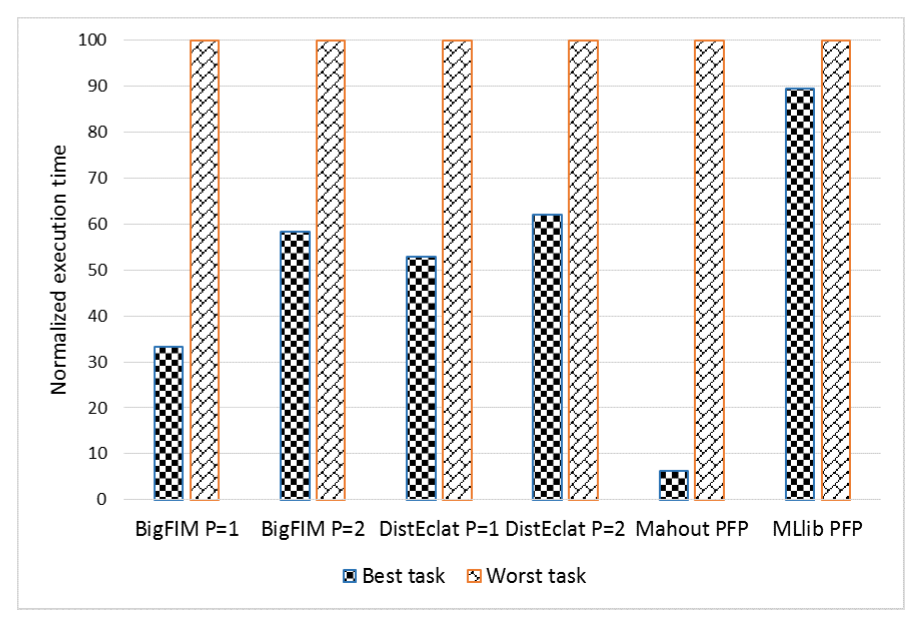
\includegraphics[width=5in]{immagini/load_balance_big_2.eps}
\caption{Normalized execution time of the most unbalanced tasks.}
\label{load_balance_big}
\end{center}
\end{figure*}

%\begin{figure*}[!t]
%\begin{center}
%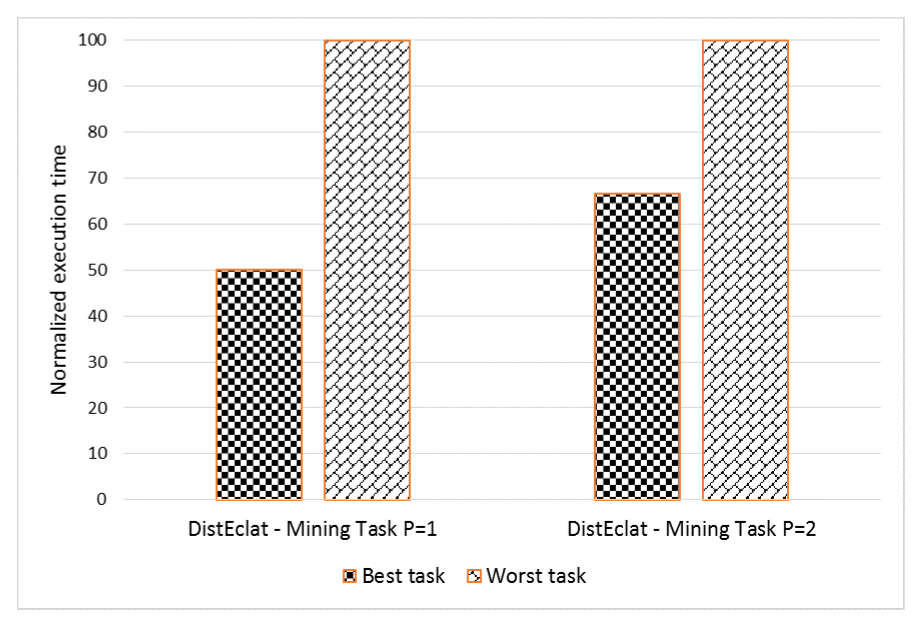
\includegraphics[width=5in]{immagini/load_balance_disteclat.eps}
%\caption{Normalized execution time of the most unbalanced tasks of DistEclat.}
%\label{load_balance_disteclat}
%\end{center}
%\end{figure*}

%In this section, experiments address the evaluation of the load balancing
%strategies of the different approaches, an often underestimated issue
%in the distributed data mining bibliography (see Section~\ref{criteria}).
% %The reason is related to the trend to implement in distributed environment
% families of algorithms which were not designed to be distributed.
% %%An example of a bad load balance is what shown in subSection
% ~\ref{attributes_exp} with Mahout PFP: a single task, with an execution period
% more than 30 times higher to the average wallclock time, slows down the whole
% process. On the other hand, approaches such as BigFIM or DistEclat were
% developed taking into account load balance.

We analyzed load balancing on a 1-hour-long subset of the
network log dataset (Table~\ref{datasets_real}) with a fixed $minsup$ of 1\%.
We consider the most unbalanced jobs of each algorithm
and compare the execution times of the fastest and the slowest tasks.
To this aim, we are not interested in the absolute execution time,
but rather in the normalized execution times, where the slowest task is
assigned a value of 100, and the fastest task is compared to such value,
as reported in Figure~\ref{load_balance_big}.

MLlib PFP achieves the best load balancing, with comparable
execution times for all tasks throughout all nodes,
whose difference is in the order of 10\%.
Mahout PFP, instead, shows the worst load balancing issues,
with differences as high as 90\%. The difference between MLlib PFP and Mahout PFP can be correlated to the 
granularity of the subproblems. The smaller the subproblems, the better the load balancing
because their execution times are more similar. MLlib PFP allows specifying the number of partitions, i.e., of subproblems, which obviously impacts on the 
granularity of each subproblem. Hence, setting opportunely this parameter, a good load balancing result is achieved. Differently, 
Mahout PFP automatically sets the number of subproblems and the current heuristic used to set it does not seem to work well on the considered datasets
(unbalanced subproblems are generated).

We included BigFIM and DistEclat with 2 different
first-phase prefix sizes.
For these algorithms, the experiment confirms that a configuration with longer prefixes
leads to a more balanced mining tasks than a configuration with short-sized prefixes,
as mentioned in Subsection~\ref{bigfim}.
%
%For BigFIM, the experiment confirms that a configuration with longer prefixes
%leads to a more balanced mining tasks than a configuration with short-sized prefixes,
%as mentioned in Subsection~\ref{bigfim}.
%Regarding DistEclat, instead, the behavior is the opposite,
%but the values are misleading: considering only the second phase of DistEclat,
%where the trees are mined, as shown in Figure~\ref{load_balance_disteclat},
%the longer the prefixes, the more balanced the mining tasks.
%Hence, DistEclat shows a medium-balanced overall behavior with 1-sized prefixes
%(50\% difference between fastest and slowest tasks),
%a good load balancing for the second phase with 2-sized prefixes (30\% difference),
%and a bad load balancing for the first phase, which affects the overall behavior,
%leading to a final 60\% difference, due to the distribution of the prefixes to
%the different nodes, their expansion and pruning.\\



%\textbf{Discussion:} Given the results of this experiment, the main motivation behind the good performances of BigFIM across all the previous experiments, despite its first phase, is its load balancing, especially with respect to Mahout PFP. As already mentioned, unfortunately, the way used to achieve this good load balancing is critical, because it exposes the algorithm to the cons of an Apriori-like approach (i.e. higher reading and communication costs and weakness with respect to dense problems). 


\subsection{Communication costs}
\label{communication_costs}

\begin{figure*}[!t]
\begin{center}
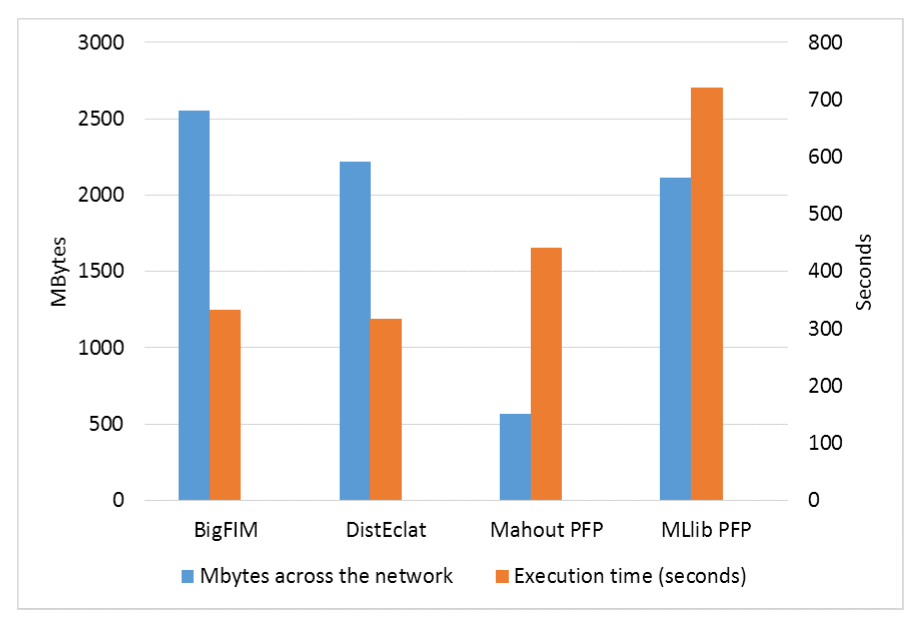
\includegraphics[width=5in]{immagini/comm_costs.eps}
\caption{Communication costs and performance for each algorithm,
Datasets~\#1, $minsup$~0.1\%.
The graph reports an average between transmitted and reveiced data.}
\label{comm_costs}
\end{center}
\end{figure*}

%\begin{table*}[h!]
%\begin{center}
%\caption{Execution times for the experiments in Figure~\ref{comm_costs},
%Datasets~\#1, $minsup$~0.1\%.}
%\label{time_comm_costs}
%\begin{tabular}{|c|c|}
%\hline
%{\bf Algorithm }& {\bf Execution time (seconds)}  \\ \hline
% \hline
%BigFIM & 332\\  \hline
%DistEclat &  317 \\ \hline
%Mahout PFP  &442\\ \hline
%MLlib PFP &  614 \\ \hline
%
%\end{tabular}
%\end{center}
%\end{table*}

%\begin{figure*}[!t]
%\begin{center}
%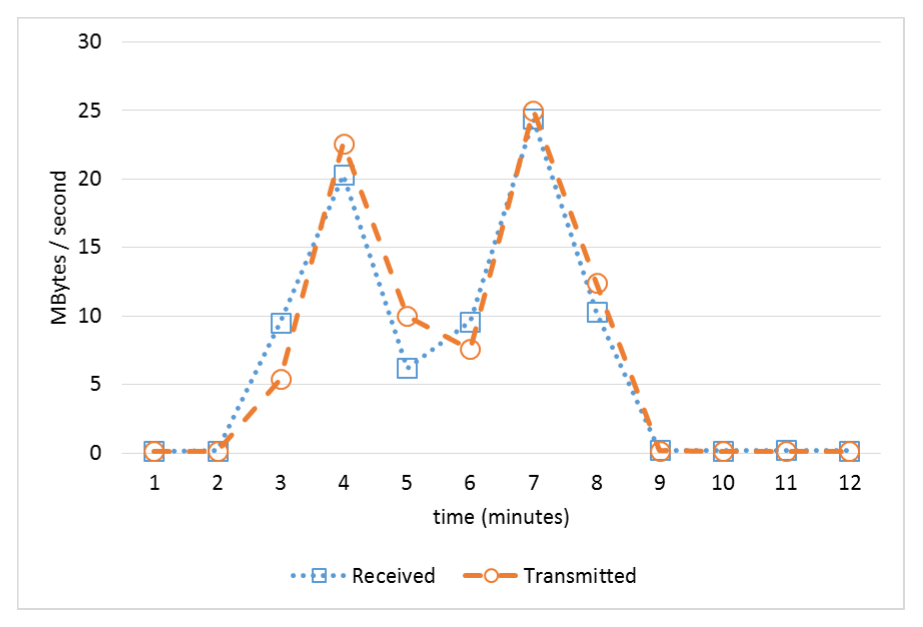
\includegraphics[width=5in]{immagini/comm_costs_bigfim.eps}
%\caption{Communication costs of BigFIM, Datasets~\#1, $minsup$~0.1\%.
%The graph reports both transmitted and reveiced data.}
%\label{comm_costs_bigfim}
%\end{center}
%\end{figure*}
%
%\begin{figure*}[!t]
%\begin{center}
%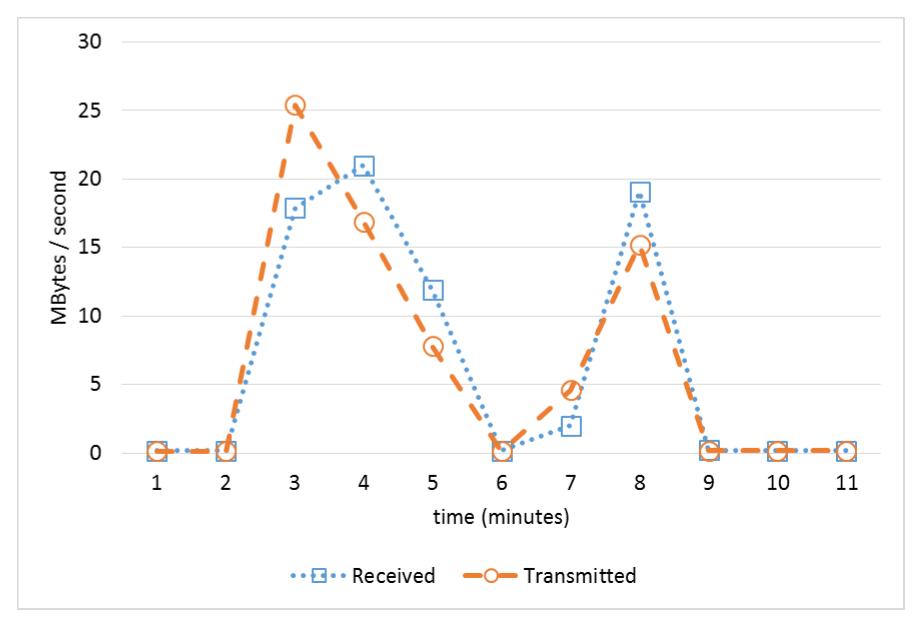
\includegraphics[width=5in]{immagini/comm_costs_disteclat.eps}
%\caption{Communication costs of DistEclat, Datasets~\#1, $minsup$~0.1\%.
%The graph reports both transmitted and reveiced data.}
%\label{comm_costs_disteclat}
%\end{center}
%\end{figure*}
%
%\begin{figure*}[!t]
%\begin{center}
%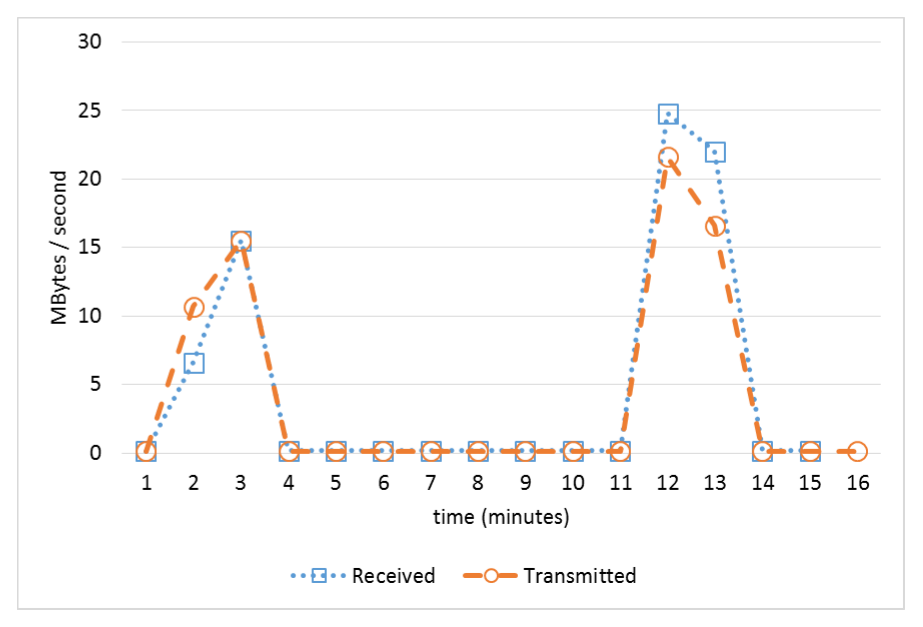
\includegraphics[width=5in]{immagini/comm_costs_mllib.eps}
%\caption{Communication costs of MLlib PFP, Datasets~\#1, $minsup$~0.1\%.
%The graph reports both transmitted and reveiced data.}
%\label{comm_costs_mllib}
%\end{center}
%\end{figure*}
%
%\begin{figure*}[!t]
%\begin{center}
%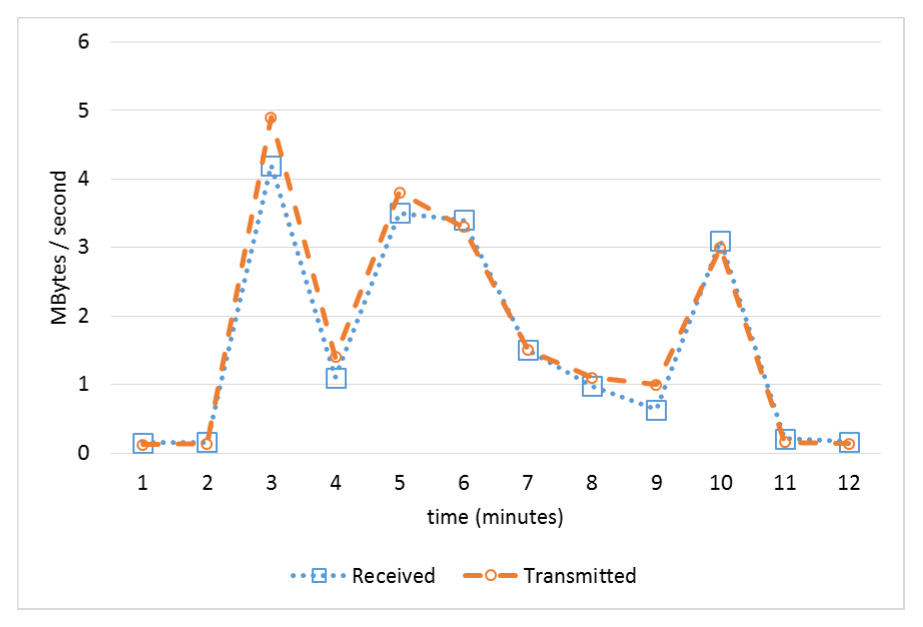
\includegraphics[width=5in]{immagini/comm_costs_pfp.eps}
%\caption{Communication costs of Mahout PFP, Datasets~\#1, $minsup$~0.1\%.
%The graph reports both transmitted and reveiced data.
%}
%\label{comm_costs_pfp}
%\end{center}
%\end{figure*}




To evaluate the communication cost, we measure the amount of data transmitted and received
through the nodes network interfaces. This information has been retrieved
by means of the utilities provided by the Cloudera Manager tool.

The experiments have been performed on Dataset~\#1 with a fixed $minsup$ value of 0.1\%,
which was the lowest value for which all algorithms completed the extraction.
Figure~\ref{comm_costs} reports, for each algorithm, the average value
among transmitted and received traffic, compared to the total execution time.
Firstly, the two measures do not seem to be correlated:
higher communication costs are associated with low execution times
for BigFIM and DistEclat, whereas MLlib reports both measures with high values.
Mahout PFP has a communication cost 4 to 5 times lower than all the others,
which exchange an average of 2~Gigabytes of data.
Mahout PFP average communication cost is around 0.5~Gigabytes,
which is approximately the dataset size.
The difference between DistEclat and BigFIM is not large because with only 2-length prefixes just an extra iteration is done by BigFIM.
Even though Mahout PFP is the most communication-cost optimized implementation,
the very low amount of data sent through the network is related
to the adoption of compression techniques, which lead to higher execution times.
%To address this issue,
%we measured the communication costs of the first phase of BigFIM and Mahout PFP
%in word-count toy application. 
%BigFIM generates into the network an
%amount of data more than 5 times larger than Mahout PFP.
%However, at the same time, the execution time of BigFIM initial phase is
%almost 3 times faster than those of Mahout PFP.

%\textbf{Discussion: }These results are consistent with the aformentioned direction. Load Balancing and Communication costs, the main issues in distributed algorithm environment, in this specific scenario do not have the same impact. On the contrary, while the communication costs analysis could be misleading if compared with wall-clock time performances, the behavior of the algorithms in terms of load balancing respect the execution time ranking. We specifically mean MLlib PFP, often the most performant approach, and Mahout PFP, in some experiments unexpectedly outperformed by algorithms theoretically slower. 



\subsection{Discussion}

Experiments confirm that performance of the data-split-based algorithms
(i.e., BigFIM in its first phase) is highly affected by the number of candidate itemsets, 
which must be stored in the temporary main memory of each task. 
Specifically, BigFIM crashes during its Apriori-based phase when low $minsup$ values or dense datasets are considered,
due to the large number of generated candidate itemsets. 
This issue does not affect the approaches based on the search split strategy (Mahout PFP and MLlib PFP), 
since they do not need to store candidate itemsets as an intermediate result.
Hence, Mahout PFP and MLlib PFP proved to be more suitable than BigFIM to process large dataset sizes, high-density datasets, and low $minsup$ thresholds. 
DistEclat deserves a separate consideration: even if it is based on the search space approach, 
it often runs out of memory,
because in its initial job it needs to store the $tidlists$ of all frequent items in main memory 
and this operation becomes easily unfeasible when large or dense datasets are considered. 
%Hence, DistEclat is exploitable only when relatively small datasets are considered and in that condition it is also the faster algorithm.

Experiments also highlight the predominant importance of load balancing in the itemset mining problem, 
in particular when comparing BigFIM to Mahout PFP. 
Since the initial mining phase of BigFIM is based on the data split parallelization approach,
it reads many times the input dataset (differently than Mahout PFP).
Moreover, BigFIM is also characterized by greater communication costs than Mahout PFP. 
These two factors should impact significantly on the execution time of BigFIM. 
Instead, 
not only the execution time of BigFIM is comparable with that of Mahout PFP 
with 1000-million record datasets (Figure~\ref{transactions}),
but BigFIM is also even faster than Mahout PFP in specific cases, e.g., 
with datasets with an average number of items per transaction greater than 70 (Figure~\ref{attributes}).
The rationale of 	such results is the better load balancing of BigFIM with respect to Mahout PFP. 
Results highlight that load balancing seems to be predominant than the number of dataset reads (I/O costs) and communication costs in the parallelization of the itemset mining problem.





%\textbf{DA RIMUOVERE, confermato (Daniele). Discussion (Versione preparata da Fabio. Da Eliminare una volta verificato che non ci sia qualche parte interessante che non ho riportato nella nuova versione}
%
%In Section~\ref{minsup_exp}, measuring the impact of \textbf{minsup threshold}, we have seen that, as expected, the first phase of BigFIM is fundamental for its scalability. 
%It represents the failure point when the number of candidate itemsets is too large to be stored in the main memory of the mappers. 
%At the same time, thanks to the better load balancing, given by the split of the mining in two balanced phases, BigFIM is able to achieve overall competitive performances (when it does not run out of memory in the first phase). While the failures related to mining tasks characterized by deep search space exploration was expected, because of the weakness of breadth-first approach with respect to data density, for the same reasons, the good performances of BigFIM in terms of execution time were less expected. Probably, the competitive performances were caused by the better load balancing in the search space exploration partitioning.
%
%DistEclat runs easily out of memory because of the size of the input dataset,
%which is transposed in a vertical format during the first phase. 
%The longer tidlists prevent it from completing such step. Even for this algorithm, the first phase is critical. The assumption of storing almost all the input dataset in all the nodes, at the aim of saving reading phases and communication costs, revealed to be not suitable for a problem characterized by a deep search space exploration.
%
%Mahout PFP and MLlib PFP are the only algorithms
%to complete the mining tasks for all $minsup$ values.
%Precisely, Mahout PFP is the most suitable technique
%when dealing with minsup values over 0.05\%,
%with a performance 6 to 8 times faster than the MLlib sibling.
%However, with lower $minsup$ values,
%Spark MLlib becomes the fastest approach with an order of magnitude gap.
%We identified the cause of the different performance
%between the two PFP implementations
%in the different pruning strategies.
%The algorithms which extract closed itemsets, such as Mahout PFP,
%can apply more effective pruning techniques
%that are not applicable when all frequent itemsets must be extracted,
%which is the case for MLlib PFP.
%When the problem becomes deeper and more challenging, beyond the engineering differences between the two implementations, the better load balancing of the MLlib PFP makes it faster.
%
%In Section~\ref{attributes_exp}, instead, we have measured the impact of \textbf{the length of the transactions} on the mining performances. As expected (see Figure~\ref{attributes_deeper}), for more dense data distributions the number of candidate itemsets increases and BigFIM runs out of memory due to its initial Apriori phase. 
%A similar motivation holds for DistEclat failures, due to its requirement to store all the (longer) tidlists in all the nodes.
%The FP-growth based approaches are affected by the increasing length of the transactions. However, their depth-first structure revealed to be the best exploration strategy in such an environment (i.e. high number of attributes). 
%DistEclat leverages a depth-first exploration strategy as well, however it assumes that all the tidlists should be stored in all the commodity cluster nodes, which is challenging if considering the further memory requirements due to the search space exploration. 
%
%In Section~\ref{nr_machines} the \textbf{speedup} achieved by the algorithms with different \textbf{degrees of parallelization} is evaluated. Based on the results it is clear that many of the considered algorithms are not able to properly exploit the parallelism provided by distributed frameworks. The reason 
%is probably given by the fact that they are not able to split the initial problem in a number of subproblems equal to the number of available parallel 
%tasks, or, when they are able to do so, the overhead given by the instance of the subtasks is greater than the advantages given by the parallel execution 
%of the subtasks/subproblems.
%
%\textbf{Load balance}, one the most important distributed features, is evaluated in Section~\ref{load_exp}.
% Given the results of this experiment, the main motivation behind the good performances of BigFIM across all the previous experiments, despite its first phase, is its load balancing, especially with respect to Mahout PFP. 
%As already mentioned, unfortunately, the way used to achieve this good load balancing is critical, because it exposes the algorithm to the cons of an Apriori-like approach (i.e. higher reading and communication costs and weakness with respect to dense problems). 
%
%Finally, Section~\ref{communication_costs}, analyzes the \textbf{communications costs} related to the mining, in terms of data transmitted in the commodity cluster network. These results suggest that Load Balancing and Communication costs, the main issues in distributed algorithm environment, in this specific scenario do not have the same impact. On the contrary, while the communication costs analysis could be misleading if compared with wall-clock time performances, the behavior of the algorithms in terms of load balancing respects the execution time ranking. For instance, Mahout PFP, in some experiments is unexpectedly outperformed by algorithms with higher communication costs. 
%
%


%\textbf{Discussion (Fabio: Recap di tutte le discussion precedenti che sono state commentate)}
%
%In Section~\ref{minsup_exp}, measuring the impact of \textbf{minsup threshold}, we have seen that, as expected, the first phase of BigFIM is fundamental for its scalability. 
%It represents the failure point when the number of candidate itemsets is too large to be stored in the main memory of the mappers. 
%At the same time, thanks to the better load balancing, given by the split of the mining in two balanced phases, BigFIM is able to achieve overall competitive performances (when it does not run out of memory in the first phase). While the failures related to mining tasks characterized by deep search space exploration was expected, because of the weakness of breadth-first approach with respect to data density, for the same reasons, the good performances of BigFIM in terms of execution time were less expected. Probably, the competitive performances were caused by the better load balancing in the search space exploration partitioning.
%
%DistEclat runs easily out of memory because of the size of the input dataset,
%which is transposed in a vertical format during the first phase. 
%The longer tidlists prevent it from completing such step. Even for this algorithm, the first phase is critical. The assumption of storing almost all the input dataset in all the nodes, at the aim of saving reading phases and communication costs, revealed to be not suitable for a problem characterized by a deep search space exploration.
%
%Mahout PFP and MLlib PFP are the only algorithms
%to complete the mining tasks for all $minsup$ values.
%Precisely, Mahout PFP is the most suitable technique
%when dealing with minsup values over 0.05\%,
%with a performance 6 to 8 times faster than the MLlib sibling.
%However, with lower $minsup$ values,
%Spark MLlib becomes the fastest approach with an order of magnitude gap.
%We identified the cause of the different performance
%between the two PFP implementations
%in the different pruning strategies.
%The algorithms which extract closed itemsets, such as Mahout PFP,
%can apply more effective pruning techniques
%that are not applicable when all frequent itemsets must be extracted,
%which is the case for MLlib PFP.
%When the problem becomes deeper and more challenging, beyond the engineering differences between the two implementations, the better load balancing of the MLlib PFP makes it faster.
%
%In Section~\ref{attributes_exp}, instead, we have measured the impact of \textbf{the length of the transactions} on the mining performances. As expected (see Figure~\ref{attributes_deeper}), for more dense data distributions the number of candidate itemsets increases and BigFIM runs out of memory due to its initial Apriori phase. 
%A similar motivation holds for DistEclat failures, due to its requirement to store all the (longer) tidlists in all the nodes.
%The FP-growth based approaches are affected by the increasing length of the transactions. However, their depth-first structure revealed to be the best exploration strategy in such an environment (i.e. high number of attributes). 
%DistEclat leverages a depth-first exploration strategy as well, however it assumes that all the tidlists should be stored in all the commodity cluster nodes, which is challenging if considering the further memory requirements due to the search space exploration. 
%
%In Section~\ref{nr_machines} the \textbf{speedup} achieved by the algorithms with different \textbf{degrees of parallelization} is evaluated. Based on the results it is clear that many of the considered algorithms are not able to properly exploit the parallelism provided by distributed frameworks. The reason 
%is probably given by the fact that they are not able to split the initial problem in a number of subproblems equal to the number of available parallel 
%tasks, or, when they are able to do so, the overhead given by the instance of the subtasks is greater than the advantages given by the parallel execution 
%of the subtasks/subproblems.
%
%\textbf{Load balance}, one the most important distributed features, is evaluated in Section~\ref{load_exp}.
% Given the results of this experiment, the main motivation behind the good performances of BigFIM across all the previous experiments, despite its first phase, is its load balancing, especially with respect to Mahout PFP. 
%As already mentioned, unfortunately, the way used to achieve this good load balancing is critical, because it exposes the algorithm to the cons of an Apriori-like approach (i.e. higher reading and communication costs and weakness with respect to dense problems). 
%
%Finally, Section~\ref{communication_costs}, analyzes the \textbf{communications costs} related to the mining, in terms of data transmitted in the commodity cluster network. These results suggest that Load Balancing and Communication costs, the main issues in distributed algorithm environment, in this specific scenario do not have the same impact. On the contrary, while the communication costs analysis could be misleading if compared with wall-clock time performances, the behavior of the algorithms in terms of load balancing respects the execution time ranking. For instance, Mahout PFP, in some experiments is unexpectedly outperformed by algorithms with higher communication costs. 
%




%%\\
%\textbf{fabio: eliminerei da qui in poi}
%Investigating deeper into the specific algorithm communication-cost analisys,
%Figures~\ref{comm_costs_bigfim},~\ref{comm_costs_disteclat},~\ref{comm_costs_mllib},~\ref{comm_costs_pfp}
%show the data exchanged throughout the whole execution time
%of each algorithm.
%
%BigFIM and DistEclat, in
%Figure~\ref{comm_costs_bigfim},~\ref{comm_costs_disteclat}, have a similar
%behaviour, with the communication costs grouped into two main phases.
%The first phase is related to the prefix extraction,
%while the second one matches the prefix preparation and prefix tree mining.
%BigFIM saturates the network link capacity (25~Megabytes/s, corresponding to
%a 100~Mbit/s full duplex Ethernet interface) during the second phase peak
%at minute 7 for both sent and received data,
%whereas DistEclat reaches such point during the first phase at minute 3,
%in trasmitted data only.
%BigFIM is also continuously exchanging data through the network during the
%mining process, whereas DistEclat pauses the network data exchange at minute 6.
%% %The choice of doing the main tasks of each job (prefix mining and prefix
%% expansion) in the map phase, without a full exploitation of data locality,
%% strongly affects communication costs. On the other hand, for instance, Mahout
%% PFP first phase, in which the header table is obtained through a basic
%% WordCount, each mapper exploits data locality working on its shard of the
%% dataset.
%Also the MLlib PFP implementation (Figure~\ref{comm_costs_mllib})
%presents two phases: differently from BigFIM and DistEclat, the middle ``pause'',
%dividing the first shuffling phase and the second materialization phase,
%is very long and lasts from minute 4 to minute 11,
%it is immediately followed by a peak reaching the network capacity
%at minute 12.
%Mahout PFP communication costs, instead, (Figure~\ref{comm_costs_pfp})
%consists of three phases:
%the first is related to the counting part,
%the second one corresponds to the mining phase,
%while the last one is related to the aggregation of the results.
%The peak in network data exchange is as low as 5~Mbytes/s.
%
%
%
%%
%% %However, interestingly, the behaviour does not affect the execution time of
%% this mining experiment, in which the considered implementation is outperformed
%% by BigFIM and DistEclat as shown in Table~\ref{time_comm_costs}. The reason is
%% partially related to an unfair load balancing, sinche the longest mining task
%% lasts more than three times the execution time of the fastest ones.
%
%
%%
%%
%%\section{Lessons learned FABIO: LE  METTEREI DOPO LE OPEN ISSUES}
%%\label{lesson}
%%
%%\textbf{Da Modificare: - modificare alcuni risultati legati a bigfim;  - aggiungere per il secondo reviewer le istruzioni su quanto sia facile utilizzarli; -esplicitare meglio i failures scenario visto che li ha richiesti}
%%
%%The reported experiments provide a wide view of the different behaviours of the
%%algorithms, dealing with diverse types of problems.
%%With this section, we aim at supporting the reader
%%in a conscious choice of the most suitable approach,
%%depending on the use case at hand.
%%Pursuing this target, we measured the real-life performance
%%of the openly-available frequent-pattern mining implementations
%%for the most popular distributed platforms (i.e., Hadoop and Spark).
%%They have been tested on many different datasets
%%characterised by different values of
%%minimum support ($minsup$),
%%transaction length (dimensionality),
%%number of transactions (cardinality),
%%and dataset density,
%%besides two real-life use cases.
%%Perfomance in terms of execution time, load balancing, and communication cost
%%have been evaluated:
%%a one-table summary of the results is reported in Table~\ref{all_resume}.
%%As a result of the described experience,
%%the following general suggestions emerge:
%%
%%\begin{itemize}
%% \item
%% Without prior knowledge of dataset density, dimensionality
%% (average transaction length), and cardinality (number of transactions),
%% \textbf{Mahout PFP} is the algorithm that best guarantees
%% the mining task completion,
%% at the expense of longer execution times.
%% Mahout PFP is the only algorithm able to always reach the experimental limits.
%% Furthermore, it exchanges very few data across the network of the cluster.
%% \item
%% When the dataset size is small with respect to the available memory,
%% \textbf{DistEclat} has proven to be among the fastest approaches,
%% and also to be able to reach the lowest experimental $minsup$ values.
%% DistEclat experiments showed that it cannot scale for large or
%% high-dimensional datasets, but when it can complete the itemset extraction,
%% it is very fast.
%% \item
%% On most real-world use cases, with limited dimensionality
%% (up to 60 items per transaction on average), \textbf{MLlib PFP}
%% has proven to be the most reasonable tradeoff choice,
%% with fast execution times and optimal scalability to very large datasets.
%% \item
%% Finally, for high-dimensional datasets, \textbf{BigFIM} resulted
%% the fastest approach,
%% but it cannot cope with $minsup$ values as low as the others.
%%\end{itemize}
%%
%%\begin{table*}[h!]
%%\scriptsize
%%\begin{center}
%%\caption{
%%Summary of the limits identified by the experimental evaluation of the
%%algorithms (lowest $minsup$, maximum transaction length,
%%largest dataset cardinality).
%%The faster algorithm for each experiment is marked in bold.
%%}
%%\label{all_resume}
%%\begin{tabular}{|c|c|c|c|c|}
%%\hline
%%& Section \ref{minsup_exp} & Section \ref{minsup_exp} & Section \ref{attributes_exp}& Section  \ref{transaction_exp} \\ \hline
%%% & Transaction & Transaction& Minsup value: 1\% & Minsup value 0.4 \% \\
%%% &  length: 10 & length: 30 &  &  \\ \hline
%%% & 10M transactions & 10M transactions &  10M transactions &  Transaction length 10 \\ \hline
%%% & Dataset \#1 & Dataset &  Dataset &  Dataset \\ \hline
%%           & $minsup$ & $minsup$ & transaction  & millions of   \\
%%           &          &          & length       & transactions  \\ \hline
%%Mahout PFP & 0.002\% & 0.01\%    & 100          & 100 		\\ \hline
%%MLlib PFP  & 0.002\% & \textbf{0.01\%}   & 60		& \textbf{100} 	\\ \hline
%%BigFIM     & 0.1\%   & 0.3\%     & \textbf{100} 	& 100 		\\ \hline
%%DistEclat  & \textbf{0.002\%}& - 	 & - 		& 1 		\\ \hline
%%\end{tabular}
%%\end{center}
%%\end{table*}
%%
%%%\begin{table*}[h!]
%%%\begin{center}
%%%\caption{Experimental result summary.
%%%\textbf{@FABIO8: qui secondo me devi fare una colonna per ogni subsection sperimentale,
%%%es. colonna ``valore minimo di $minsup$, Section X.Y'' e riporti i valori limite,
%%%ecc. con le altre subsection... cos\`i invece non mi piace, non \`e immediato
%%%da capire... e poi magari metterei un asterisco sul metodo pi\`u veloce
%%%(o i due pi\`u veloci se sono molto simili) in ogni colonna.
%%%Se non \`e chiaro ci sentiamo.}
%%%}
%%%\label{all_resume}
%%%\begin{tabular}{|c|c|c|c|c|}
%%%\hline
%%%           & Transaction & Transaction& Minsup value: 1\% & Minsup value 0.4 \% \\
%%%  &  length: 10 & length: 30 &  &  \\ \hline
%%%            & 10M transactions & 10M transactions &  10M transactions &  Transaction length 10 \\ \hline
%%%Algorithm  & Lowest minsup:                           & Lowest minsup:                             & Max. transaction           & Max. number of   \\
%%%  &                       &                             &  length:           & transactions (millions):   \\ \hline
%%%Mahout PFP & 0.002 \%                                  & 0.01 \%                                   & 100                                  & 100                                         \\ \hline
%%%MLlib PFP  & 0.002 \%                                  & 0.01 \%                                   & 60                                   & 100                                         \\ \hline
%%%BigFIM     & 0.1 \%                                    & 0.3 \%                                    & 100                                  & 100                                         \\ \hline
%%%DistEclat  & 0.002 \%                                  & -                                         & -                                    & 1                                           \\ \hline
%%%\end{tabular}
%%%\end{center}
%%%\end{table*}
%
%
%
%
